\documentclass[12pt]{article}
\usepackage{spikey}
\usepackage{amsmath}
\usepackage{amssymb}
\usepackage{soul}
\usepackage{float}
\usepackage{graphicx}
\usepackage{hyperref}
\usepackage{xcolor}
\usepackage{chngcntr}
\usepackage{centernot}
\usepackage{datetime}
\usepackage[shortlabels]{enumitem}
\usepackage{booktabs}

% Set font.
\usepackage{fontspec}
 
\setmainfont{Times New Roman}
%\usepackage{mathptmx}
%\usepackage[MnSymbol]{mathspec}
%\setallmainfonts{Times New Roman}

\usepackage[margin=1truein]{geometry}
\usepackage{setspace}
\linespread{1.5}

\counterwithin{equation}{section}
\counterwithin{theorem}{section}
\counterwithin{lemma}{section}
\counterwithin{corollary}{section}
\counterwithin{proposition}{section}
\counterwithin{remark}{section}
\counterwithin{example}{section}
\counterwithin{definition}{section}

% Bib package
\usepackage{apacite}

\title{Forecasting Crude Oil Returns using News Sentiment and Machine Learning \footnote{Compile Date: \currenttime\ \today}}

\author{Tianyu Du \footnote{\texttt{tianyu.du@mail.utoronto.ca}}}

\begin{document}
	\maketitle
	\tableofcontents
	\newpage
	\section{Introduction}
	
	\section{Data}
	\paragraph{}This study involves three major datasets: i) the daily spot price of crude oil at the West Texas Intermediate (WTI), ii) news sentiment dataset from Ravenpack News Analytics (RPNA), and iii) macroeconomic indicators proxying the overall economic state.

	\subsection{The West Texas Intermediate (WTI) Crude Oil Dataset}
	\paragraph{}West Texas Intermediate market spot price (coded as DCOILWTICO in the st. Louis Federal Reserve Economic Data) has been the most commonly used price for crude oil in current literature. The dataset retrieved from the Federal Reserve Bank of St. Louis is measured on a daily level and spans from January 1986 up to the present day (citation: data series). Because of the limited availability of the RavenPack dataset, this paper focuses only on crude oil prices after January 1, 2000. Analysis of the crude oil market (citation: 40-year paper) shows the spot price is highly responsive to news and other macroeconomic shocks, which is exactly the tricky part of forecasting financial time series. If the proposed forecasting pipeline performs well on the crude dataset, such a pipeline is conceivably promising on other datasets as well.

	\par Almost all financial time series suffers from missing data problem, so is the crude oil dataset. Much existing research studying stock market datasets simply drop missing values. Instead, this paper uses an autoregressive integrated moving average (ARIMA) model to interpolate and fill missing data, so that the time gap between two consecutive observations is exactly one trading day. 

	\begin{figure}[H]
		\small
		\centering
		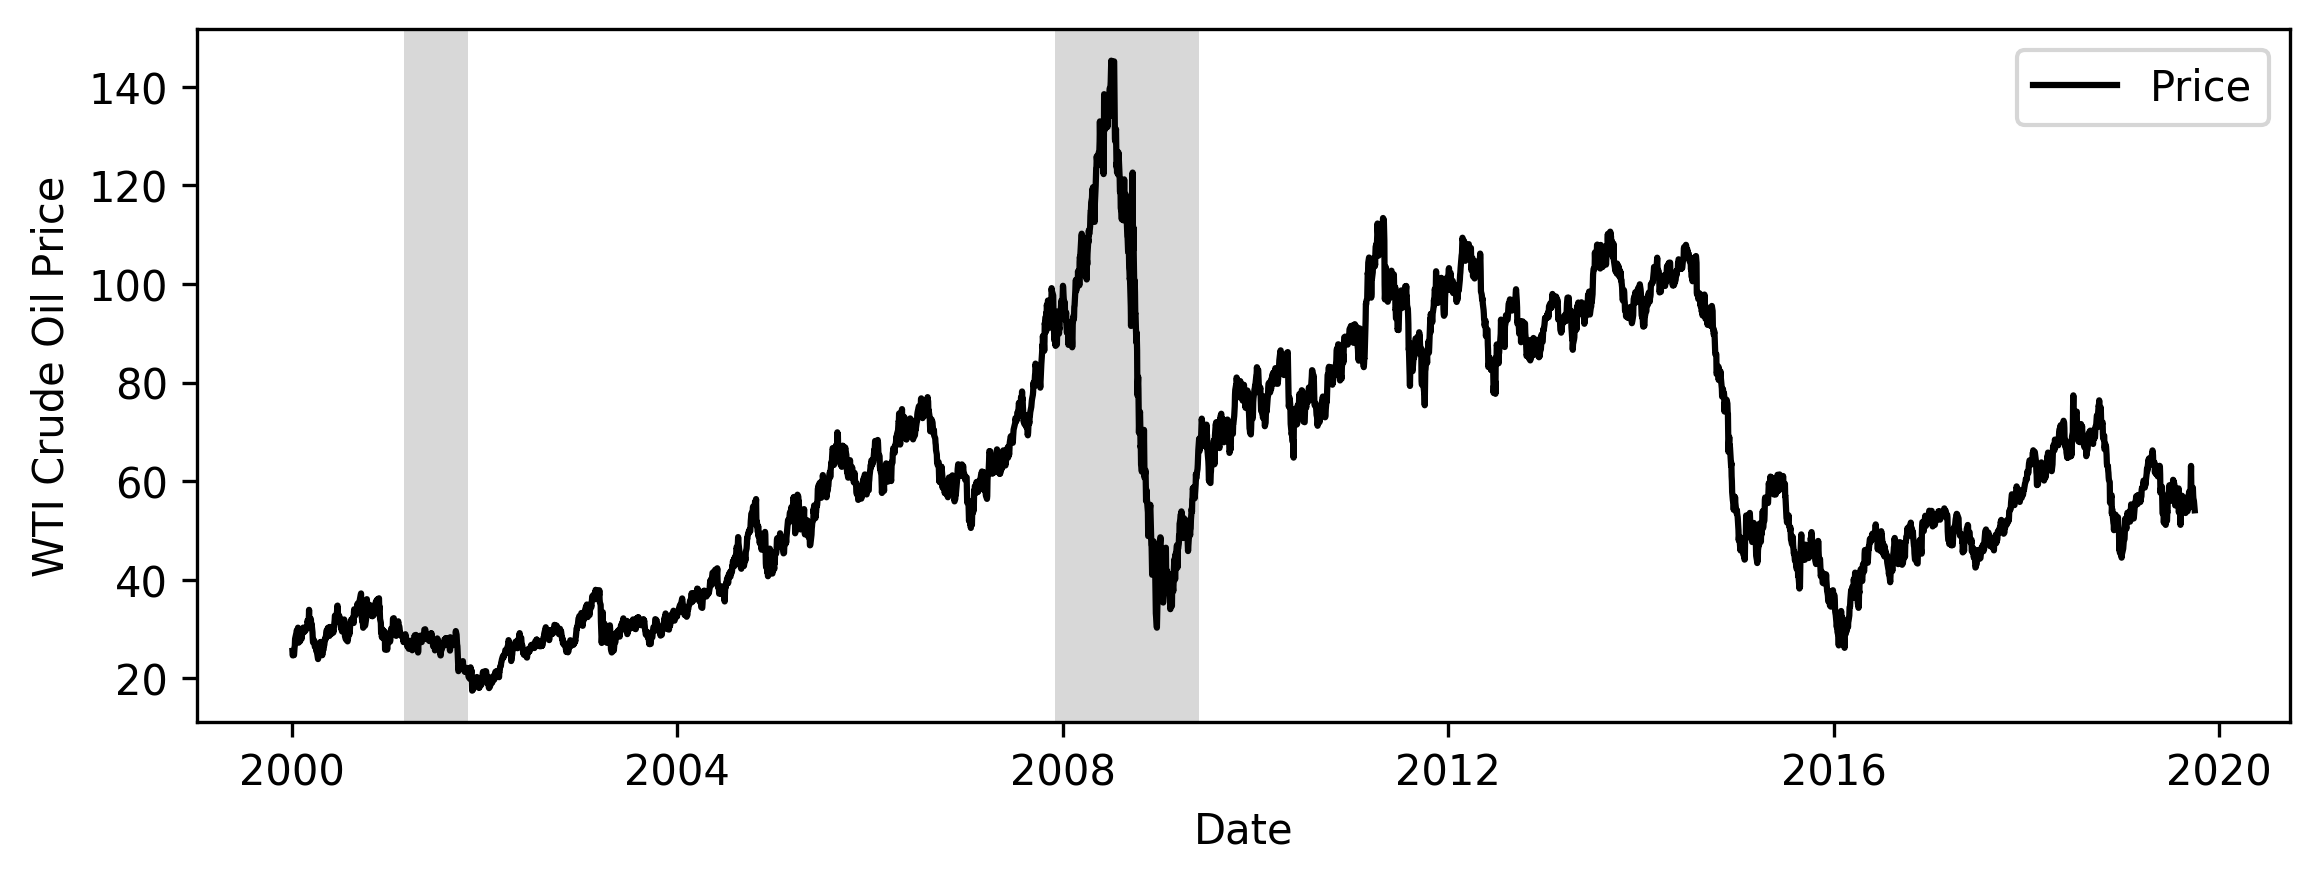
\includegraphics[width=\linewidth]{figures/wti_summary/prices.png}
		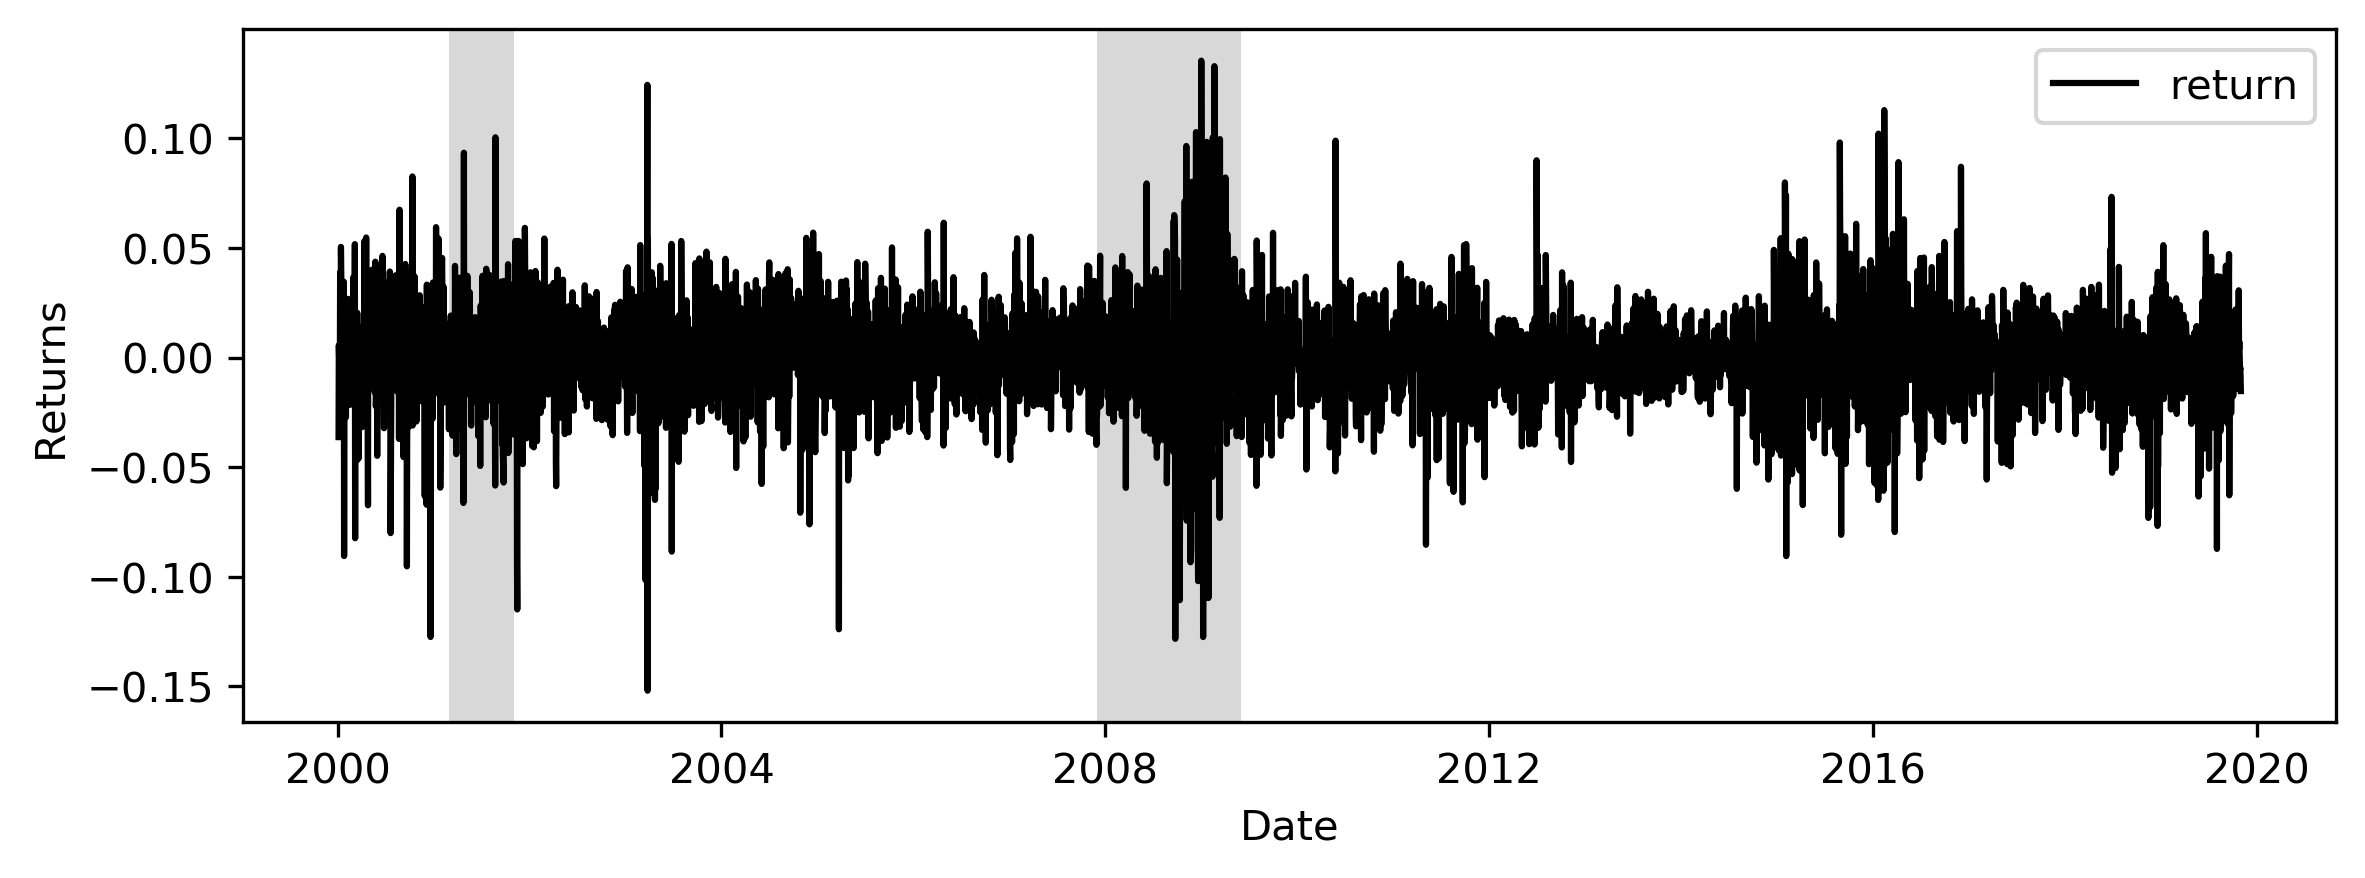
\includegraphics[width=\linewidth]{figures/wti_summary/returns.png}
		\caption{Crude oil prices and returns between January 1, 2000 and September 30, 2019. Shaded areas indicate U.S. recessions.}
	\end{figure}

	\par From the \hl{the table below} we can see that the mean return for crude oil are around zero year by year. During periods of recessions (March 2001 to November 2001 and December 2007 to June 2009), the data exhibited negative mean returns as well as relatively high standard deviations.
	\begin{table}[H]
		\small
		\centering
		\begin{tabular}{l|c c c c c c c c c}
			\toprule
			Year & Num. Obs. & Mean & Median & Std. & Min & Max & ACF(1) & ACF(3) & ACF(5) \\
			\midrule
			2000 & 249 & 0.000 & 0.004 & 0.029 & -0.127 & 0.083 & 0.012 & -0.007 & 0.126 \\
			2001 & 250 & -0.001 & -0.001 & 0.029 & -0.171 & 0.101 & 0.024 & -0.005 & -0.037 \\
			2002 & 250 & 0.002 & 0.002 & 0.021 & -0.062 & 0.060 & -0.030 & -0.008 & -0.014 \\
			2003 & 250 & 0.000 & 0.002 & 0.028 & -0.152 & 0.124 & -0.133 & 0.096 & -0.097 \\
			2004 & 249 & 0.001 & 0.003 & 0.023 & -0.076 & 0.059 & -0.074 & 0.019 & -0.036 \\
			2005 & 251 & 0.001 & 0.002 & 0.022 & -0.124 & 0.084 & -0.085 & -0.083 & -0.109 \\
			2006 & 249 & -0.000 & 0.001 & 0.018 & -0.049 & 0.062 & 0.002 & 0.008 & -0.030 \\
			2007 & 252 & 0.002 & 0.001 & 0.019 & -0.047 & 0.055 & -0.103 & 0.000 & 0.069 \\
			2008 & 253 & -0.003 & -0.001 & 0.039 & -0.128 & 0.164 & 0.008 & 0.165 & -0.259 \\
			2009 & 252 & 0.002 & 0.002 & 0.034 & -0.127 & 0.133 & -0.034 & 0.096 & -0.022 \\
			2010 & 252 & 0.001 & 0.000 & 0.019 & -0.052 & 0.099 & 0.051 & -0.071 & 0.057 \\
			2011 & 252 & 0.000 & 0.001 & 0.022 & -0.085 & 0.086 & 0.027 & -0.003 & -0.087 \\
			2012 & 252 & -0.000 & 0.001 & 0.016 & -0.048 & 0.090 & -0.154 & 0.034 & 0.120 \\
			2013 & 252 & 0.000 & 0.001 & 0.011 & -0.035 & 0.032 & 0.045 & -0.073 & -0.153 \\
			2014 & 252 & -0.002 & -0.001 & 0.016 & -0.111 & 0.049 & -0.209 & 0.054 & -0.042 \\
			2015 & 252 & -0.001 & -0.004 & 0.029 & -0.091 & 0.098 & -0.113 & -0.106 & -0.021 \\
			2016 & 252 & 0.001 & 0.000 & 0.031 & -0.080 & 0.113 & 0.006 & -0.040 & 0.078 \\
			2017 & 250 & 0.000 & 0.003 & 0.016 & -0.056 & 0.033 & -0.017 & -0.017 & 0.076 \\
			2018 & 249 & -0.001 & 0.001 & 0.020 & -0.077 & 0.073 & -0.103 & -0.056 & 0.011 \\
			2019 & 187 & 0.001 & 0.001 & 0.023 & -0.087 & 0.142 & -0.090 & -0.039 & 0.123 \\
			\midrule
			Total & 4955 & 0.000 & 0.001 & 0.024 & -0.171 & 0.164 & -0.035 & 0.021 & -0.024 \\
			\bottomrule
		\end{tabular}
		\caption{Summary Statistics for Crude Oil Returns in each Year. Note that this dataset only include nine months of 2019.}
	\end{table}
	
	
	\begin{figure}[H]
		\small
		\centering
		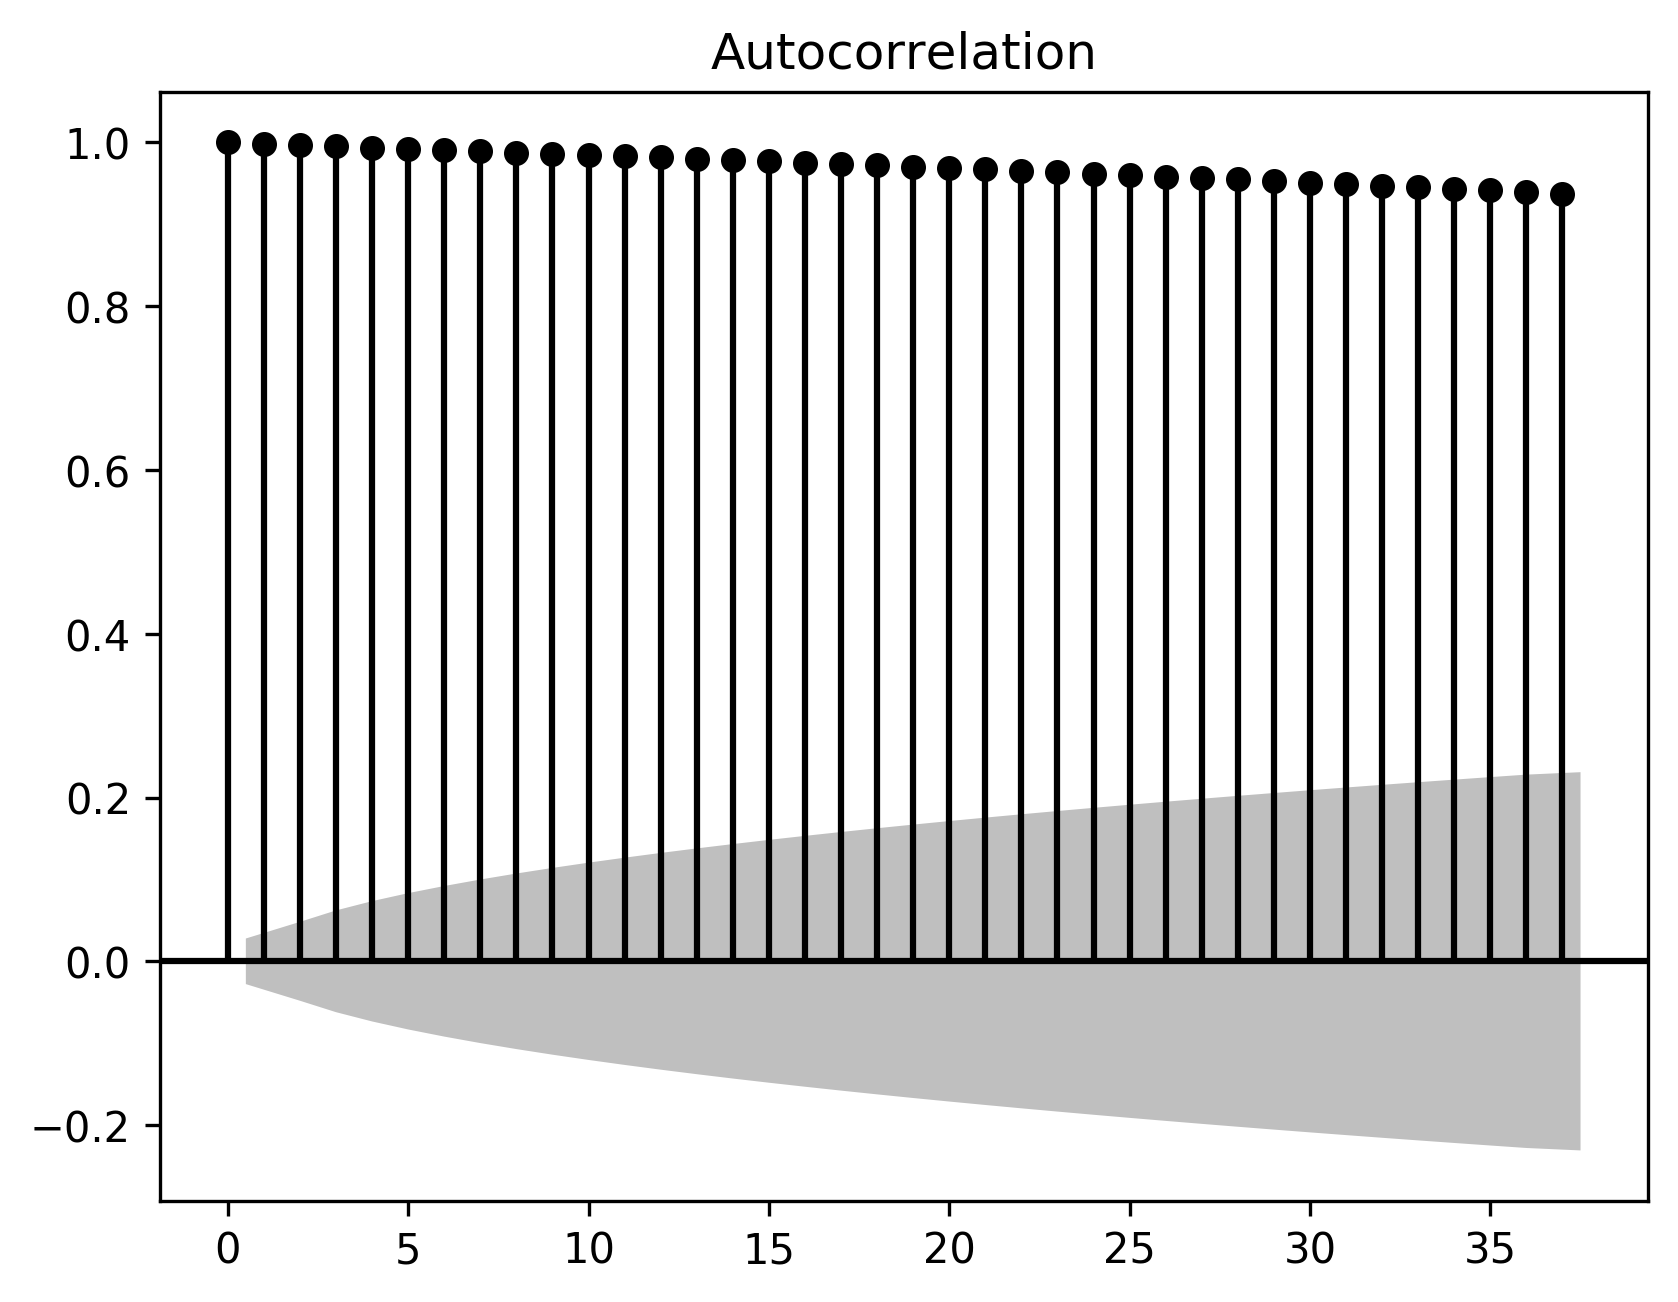
\includegraphics[width=0.45\linewidth]{figures/wti_summary/prices_acf.png}
		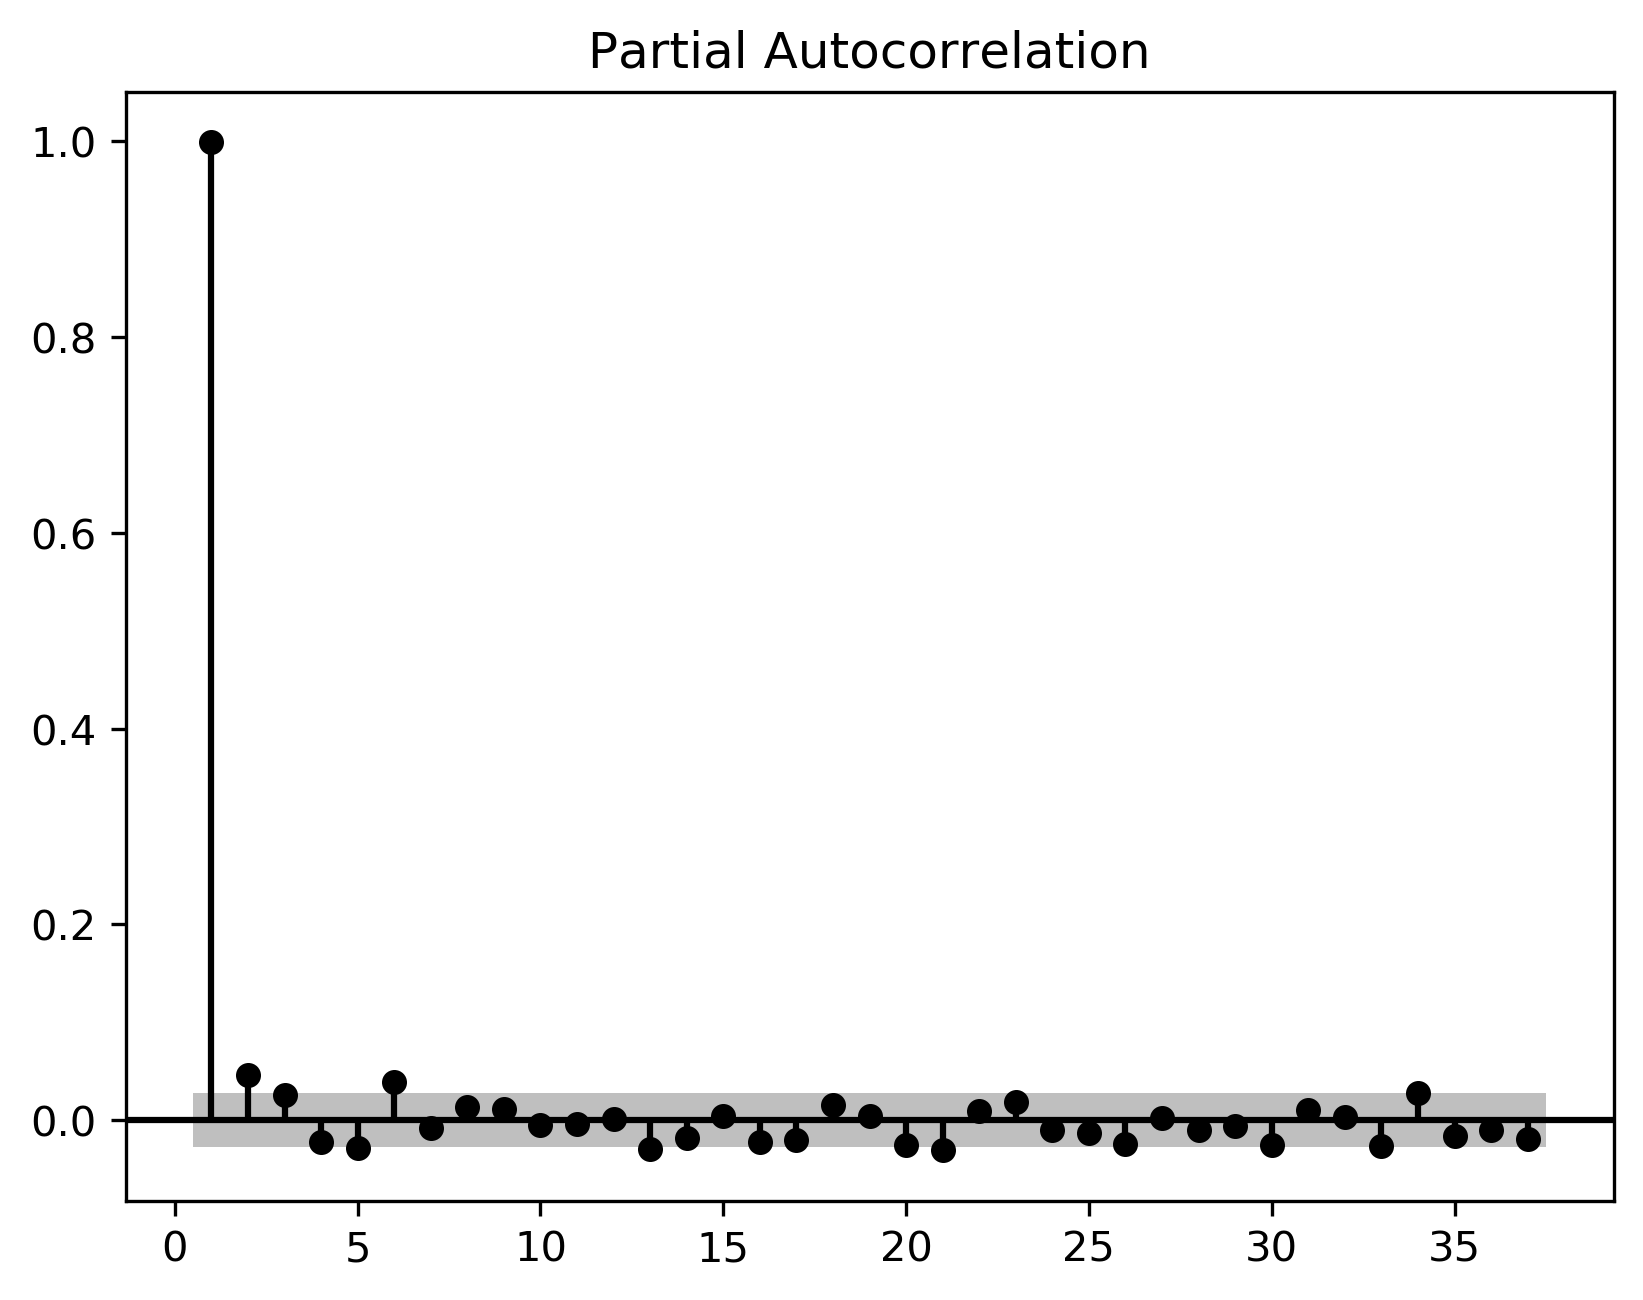
\includegraphics[width=0.45\linewidth]{figures/wti_summary/prices_pacf.png}
		\caption{ACF and PACF for Crude Oil Prices (January 2000 to September 2019)}
	\end{figure}

	\begin{figure}[H]
		\small
		\centering
		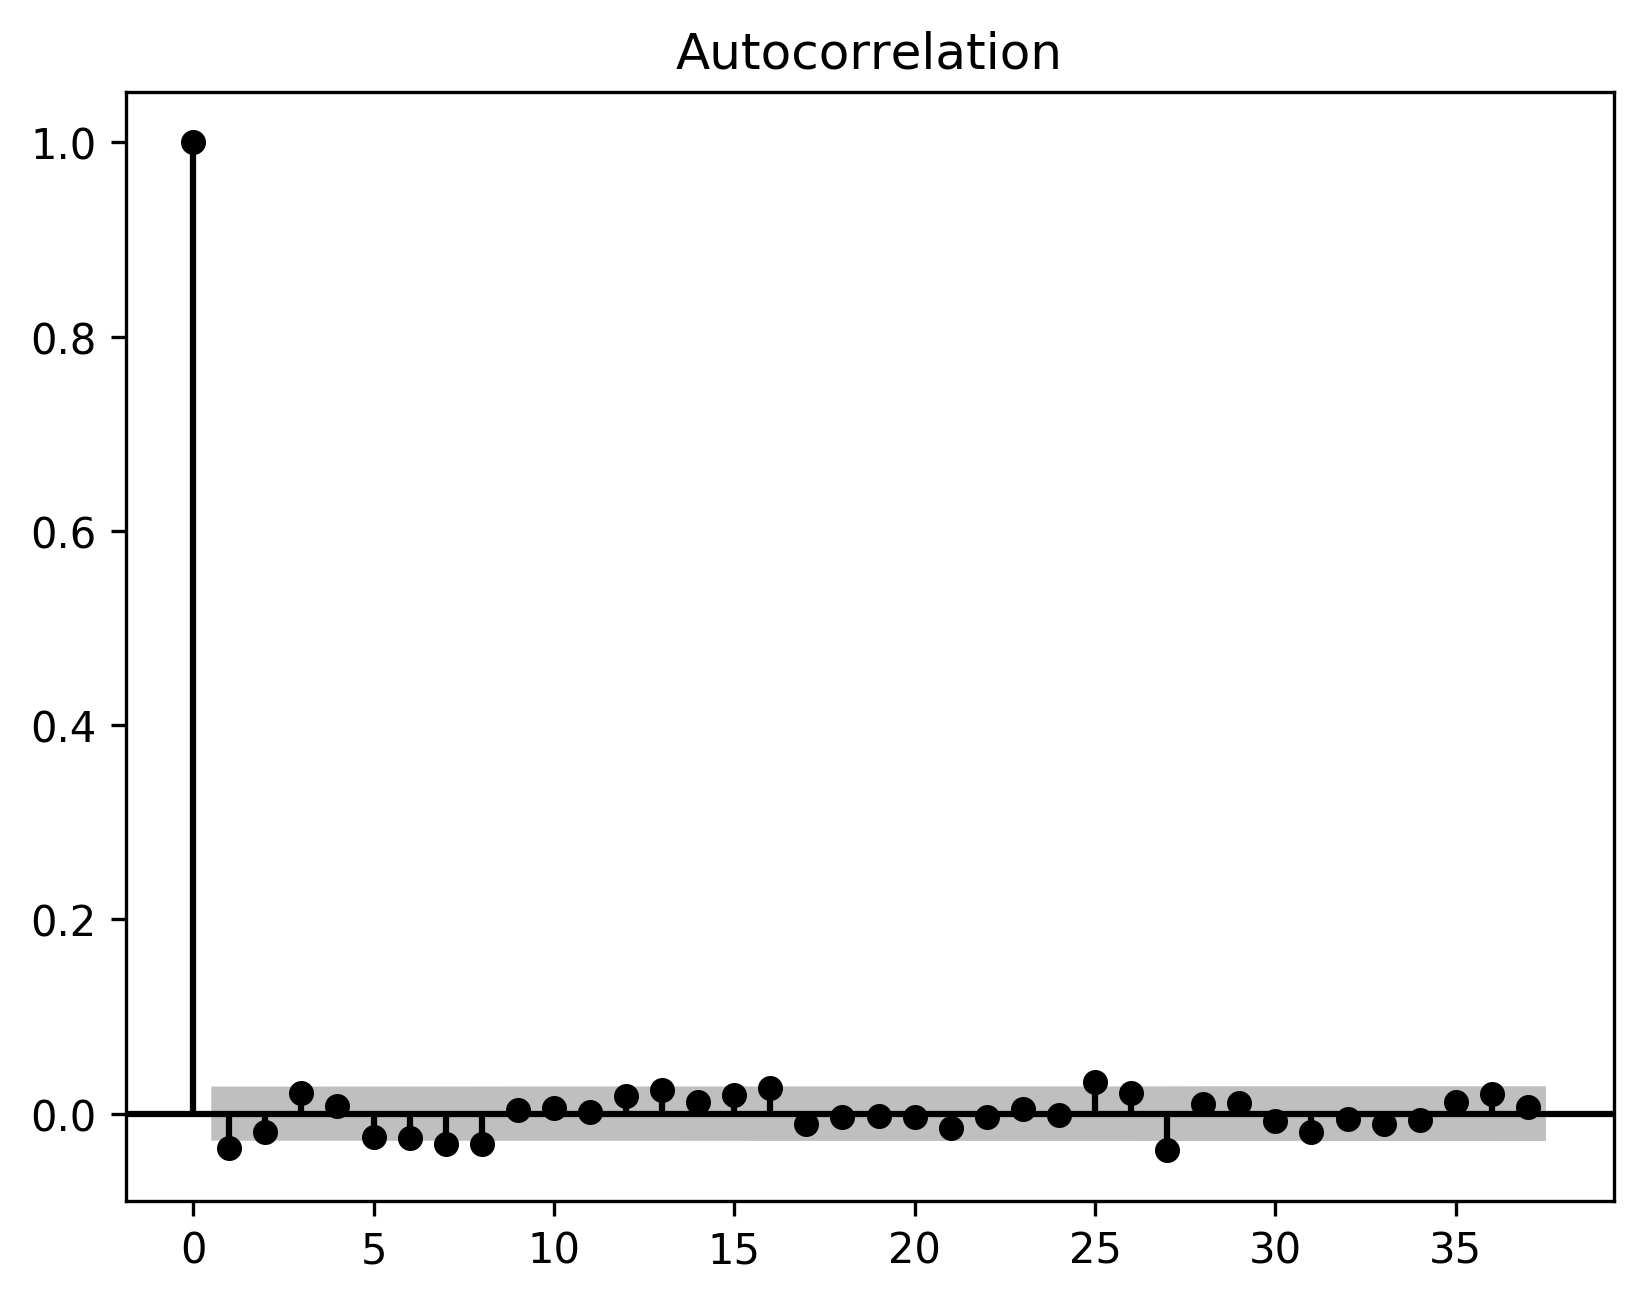
\includegraphics[width=0.45\linewidth]{figures/wti_summary/returns_acf.png}
		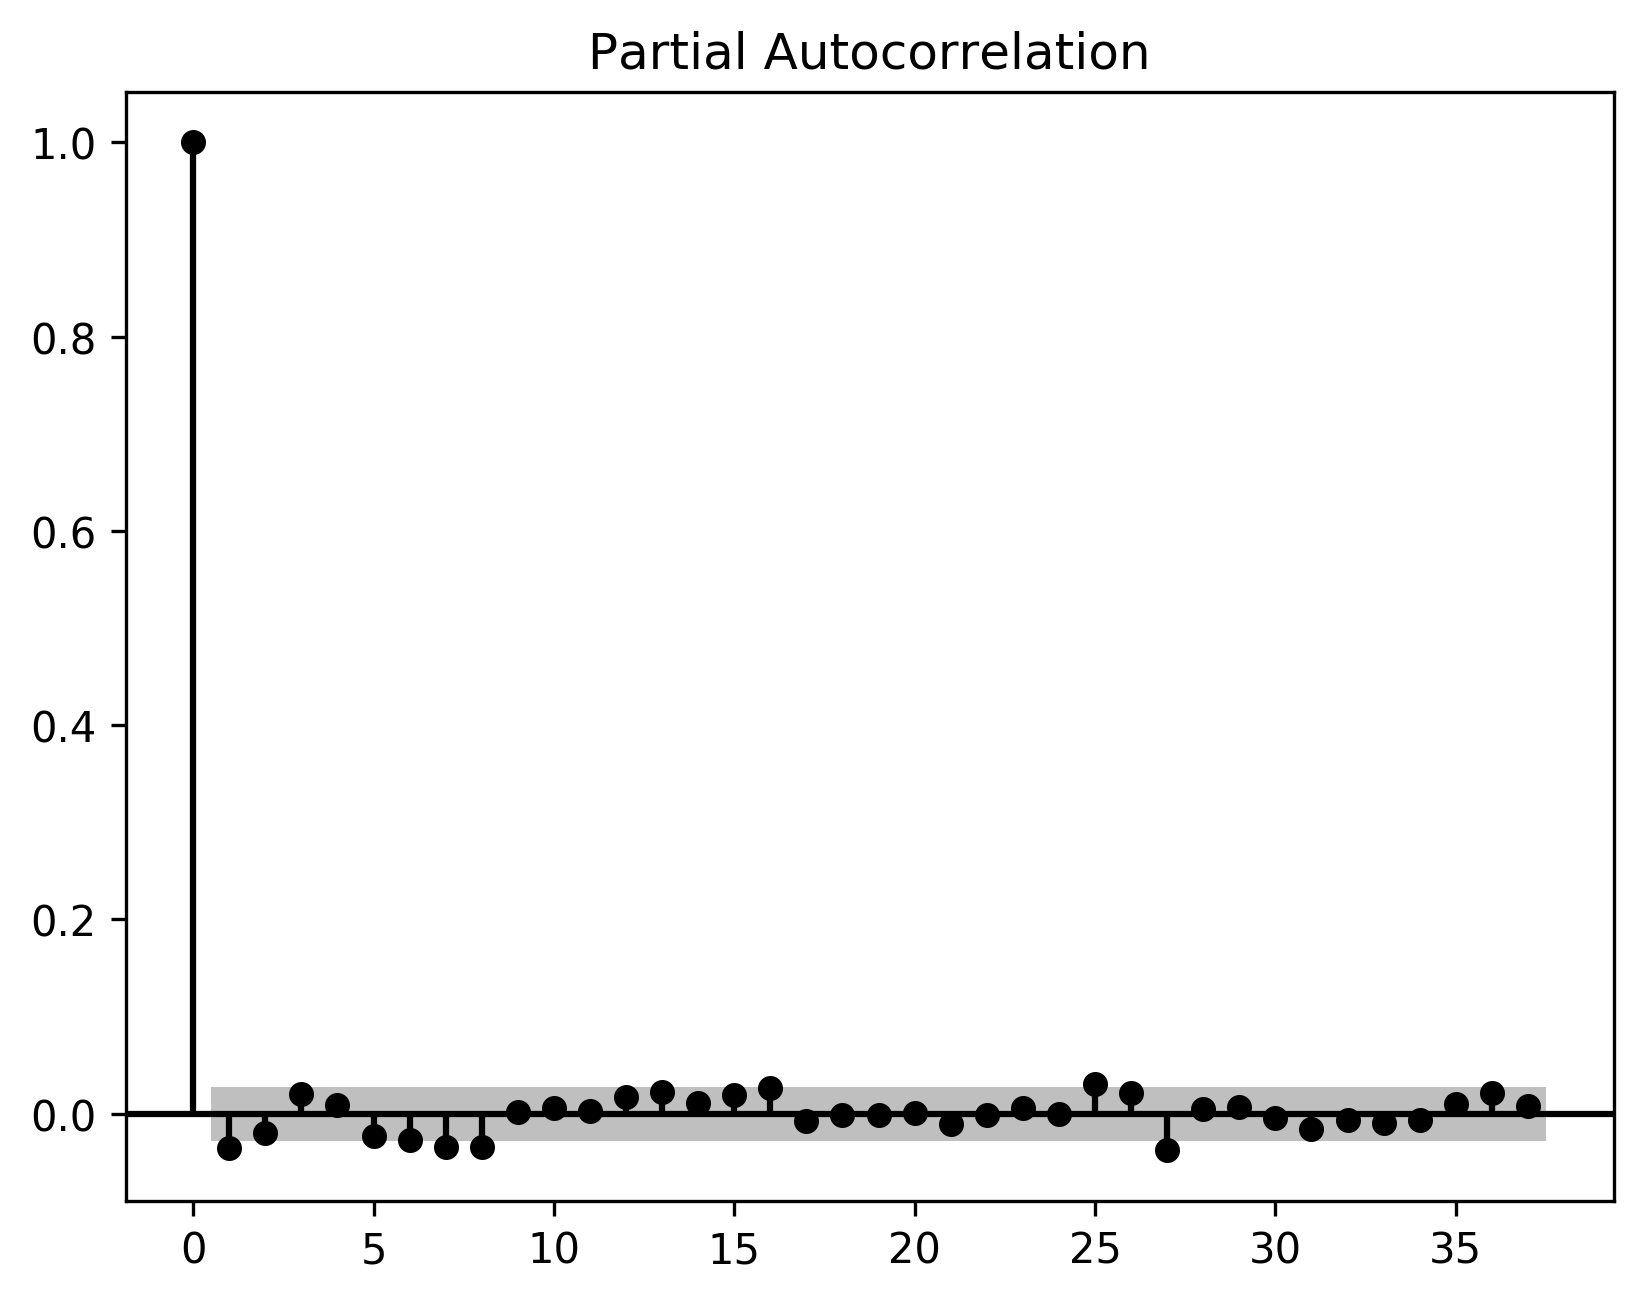
\includegraphics[width=0.45\linewidth]{figures/wti_summary/returns_pacf.png}
		\caption{ACF and PACF for Crude Oil Returns (January 2000 to September 2019)}
	\end{figure}

	\begin{figure}[H]
		\centering
		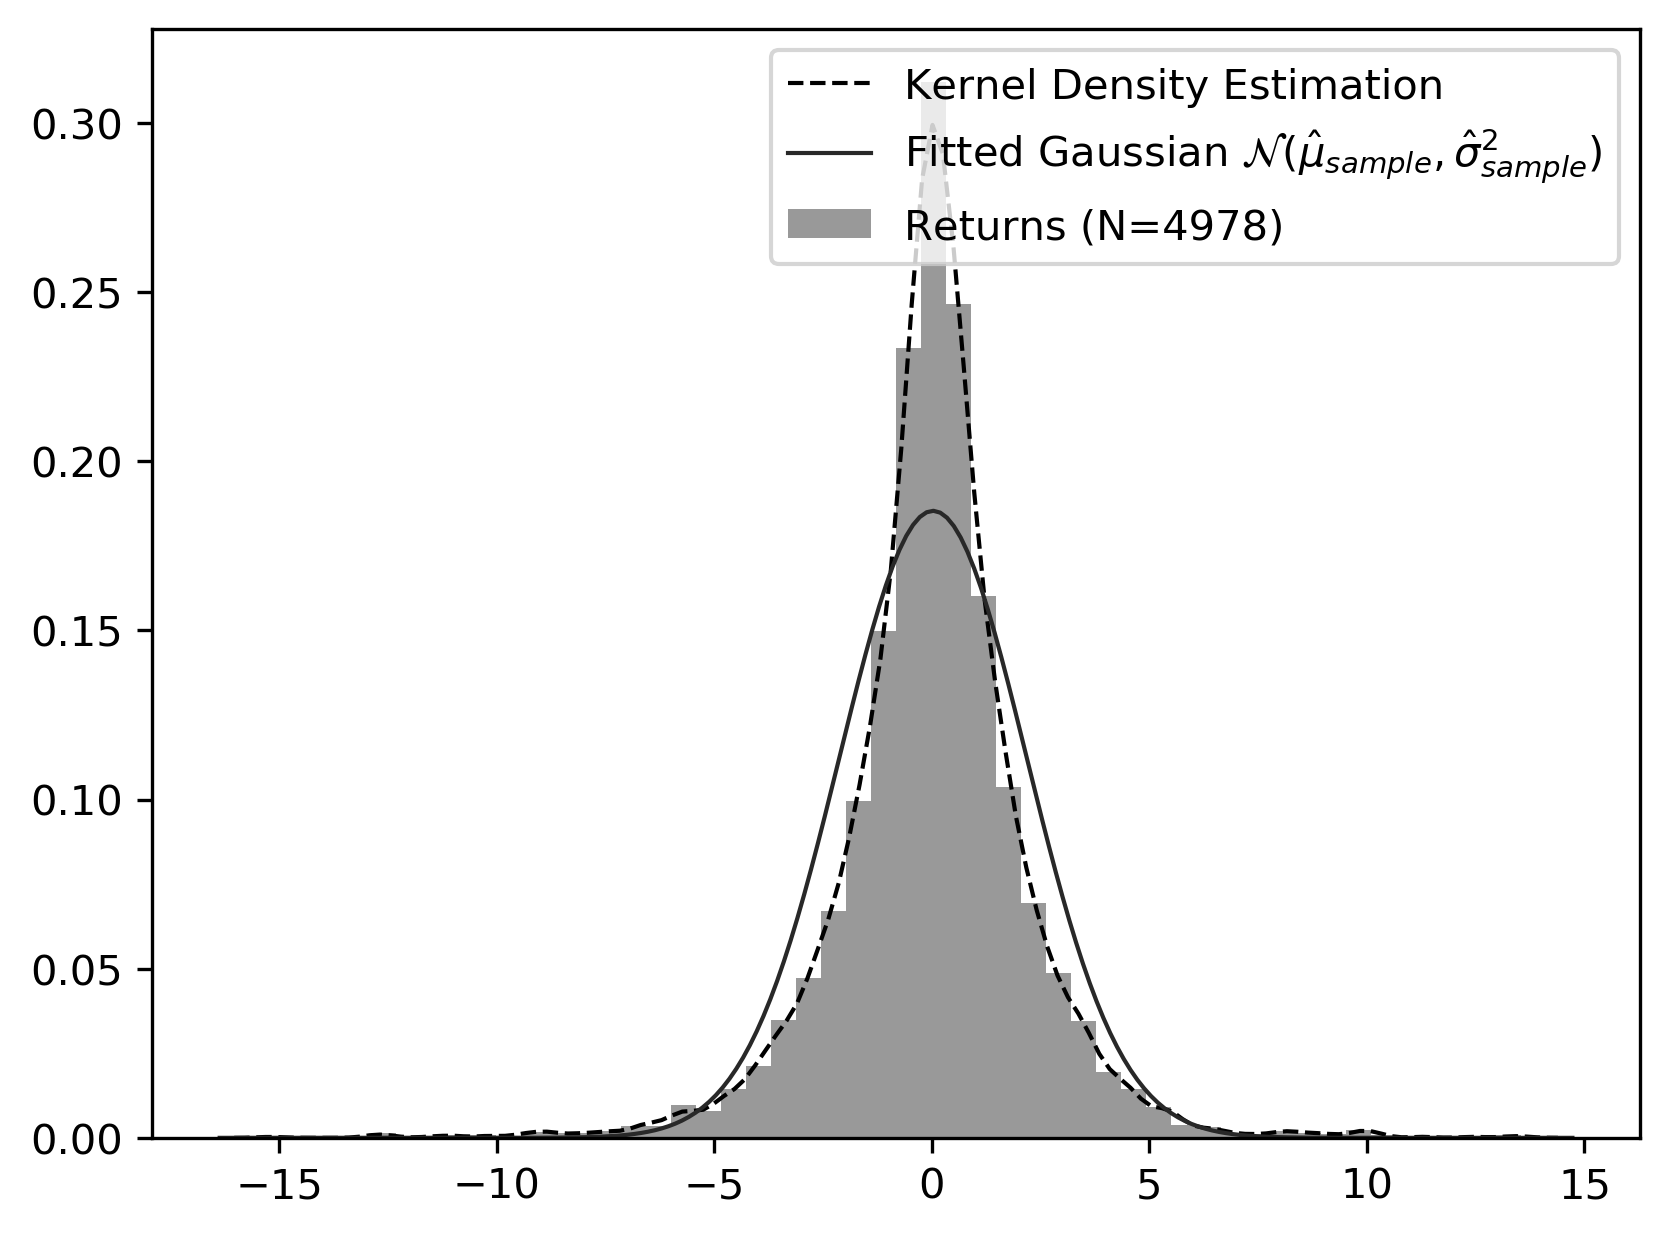
\includegraphics{figures/wti_summary/return_hist.png}
		\caption{Distribution of Crude Oil Returns (January 2000 to September 2019). KDE stands for the kernel density estimation for the empirical distribution. Gaussian fit plots the density function of $\mc{N}(\hat{\mu}_\tx{sample}, \hat{\sigma}_\tx{sample})$.}
	\end{figure}

	\subsection{Missing Data in Crude Oil Dataset}
	\paragraph{} Given the focus of this paper is on forecasting crude oil returns, which captures the difference between two consecutive prices, The missing data problem can be crucial here.

	\par This paper calculates crude oil returns on one particular day $t$ by taking the difference in logged prices at $t$ and the previous trading day:
	\begin{align}
		r_t &:= \ln(p_t) - \ln(p_{t - \Delta})
	\end{align}
	where $t - \Delta$ is the last trading day before day $t$. As mentioned before, the time gap between two observed prices are not even. For instance, the return on a Monday can be computed by taking difference between the log close price on Monday Friday (if available). In this case, $\Delta = 3$. If the previous Friday was a holiday without valid price data, $r_t$ will be $\ln(p_\tx{Mon}) - \ln(p_{\tx{Prev Thu}})$, and $\Delta = 4$. According to \hl{the table below}, 33 days are in this case.
	\begin{table}[H]
		\centering
		\small
		\begin{tabular}{l|c c c c c c c}
			\toprule
			Day of the week & Num. Days. & Num. Trading Days & $\Delta$=1 & 2 & 3 & 4 & 5 \\
			\midrule
			Monday & 1031 & 927 & 0 & 0 & 883 & 33 & 11 \\
			Tuesday & 1030 & 1018 & 921 & 0 & 0 & 97 & 0 \\
			Wednesday & 1030 & 1022 & 1011 & 5 & 0 & 0 & 6 \\
			Thursday & 1030 & 1002 & 994 & 8 & 0 & 0 & 0 \\
			Friday & 1030 & 986 & 969 & 17 & 0 & 0 & 0 \\
			Saturday & 1030 & 0 & 0 & 0 & 0 & 0 & 0 \\
			Sunday & 1030 & 0 & 0 & 0 & 0 & 0 & 0 \\
			\midrule
			Total & 7211 & 4955 & 3895 & 30 & 883 & 130 & 17 \\
			\bottomrule
		\end{tabular}
		\caption{The values of $\Delta$ used to calculate returns. This table only include trading days, but the first day with price observation in this dataset was dropped because it did not have a previous trading day, so return on this day cannot by computed using our definition.}
	\end{table}
	\par As mentioned before, the oil price dataset does not have any prices over weekends. \hl{The table below} reports dates that are most frequently associated with a missing data over the span of 20 years. The pool of days with missing data is pretty consistent overtime, the market is always closed on January 1, July 4 (Independence Day) and December 25 (Christmas). The group of dates in late November are responsible for missing data on Thanksgiving holiday.
	\begin{table}[H]
		\small
		\centering
		\begin{tabular}{l|c c}
			\toprule
			Date & Counts (all) & Counts (excl. weekends) \\
			\midrule
			July 4 & 20 & 16 \\
			January 1 & 20 & 14 \\
			December 25 & 19 & 14 \\
			July 3 & 10 & 5 \\
			November 23 & 10 & 5 \\
			November 24 & 10 & 4\\
			November 25 & 10 & 3\\
			November 22 & 9 & 4 \\
			November 26 & 9 & 3 \\
			\bottomrule
		\end{tabular}
		\caption{Dates most frequently associates with missing data. Data on January 1, July 4, and December 25 are missing ever year. Because the entire dataset ranges from January 3, 2000 to September 30, 2019, missing data problems on December 25 are only reported 19 times.}
	\end{table}
 
	\subsection{Day of the Week Effect in Crude Oil Dataset}
	\subsubsection{Difference in Returns across the Week}
	\paragraph{} Gibbons and Hess' work examined returns on stocks from S\&P 500, Dow Jones 30, and Treasury Bills. They found strong negative mean returns on Monday compared with other weekdays. The seasonality persisted even after market adjustment measures, such as using mean-adjusted returns instead, were taken \cite{Hess1981}. Analysis in this paper suggests a similar daily seasonality presents in crude oil returns as well.
	\hl{Panels in the figrure below} demonstrate the empirical distributions of returns on each day of the week. We can see that Monday and Wednesday have relatively larger variances, which again matches Gibbons and Hess' observations.
	\begin{figure}[H]
		\centering
		\small
		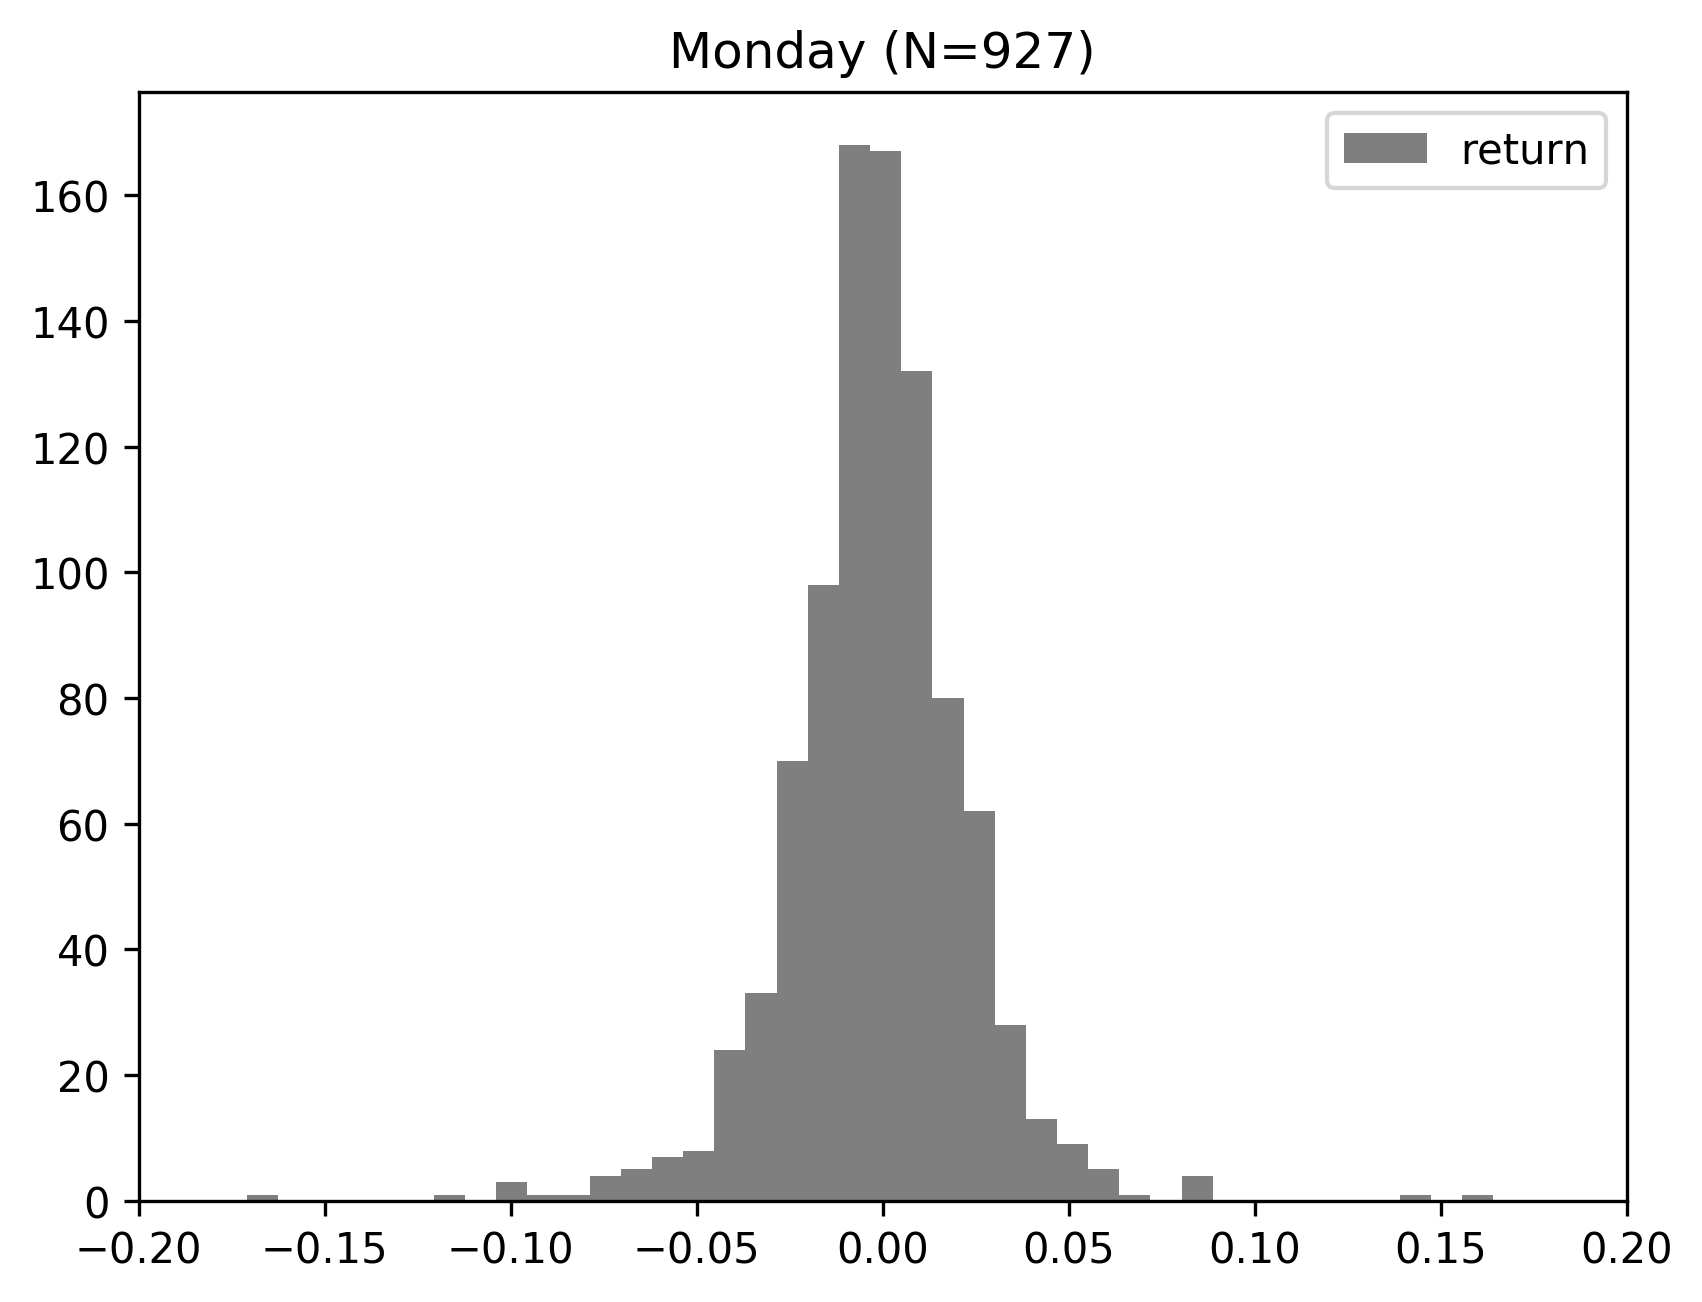
\includegraphics[width=0.45\linewidth]{figures/day_of_week_effect/dist_returns_Monday.png}
		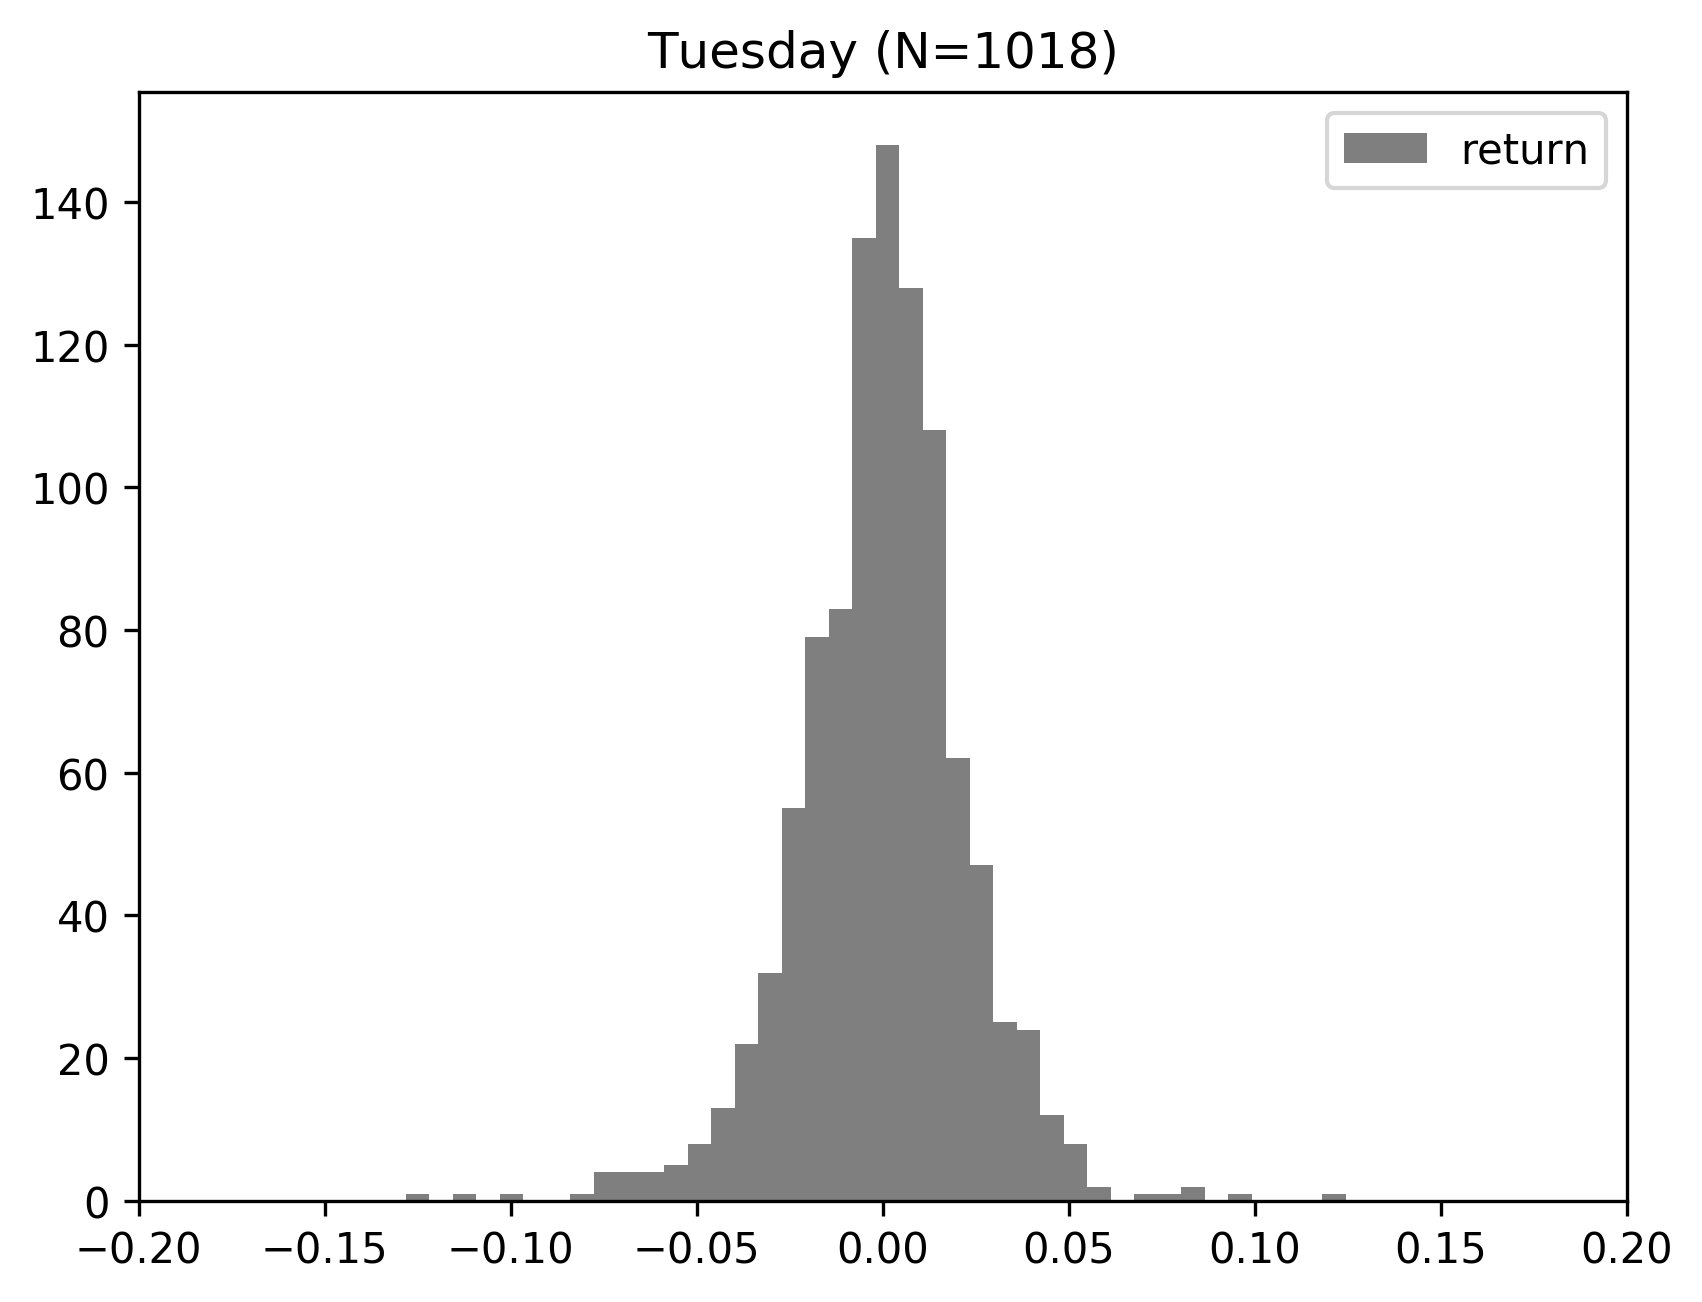
\includegraphics[width=0.45\linewidth]{figures/day_of_week_effect/dist_returns_Tuesday.png}
		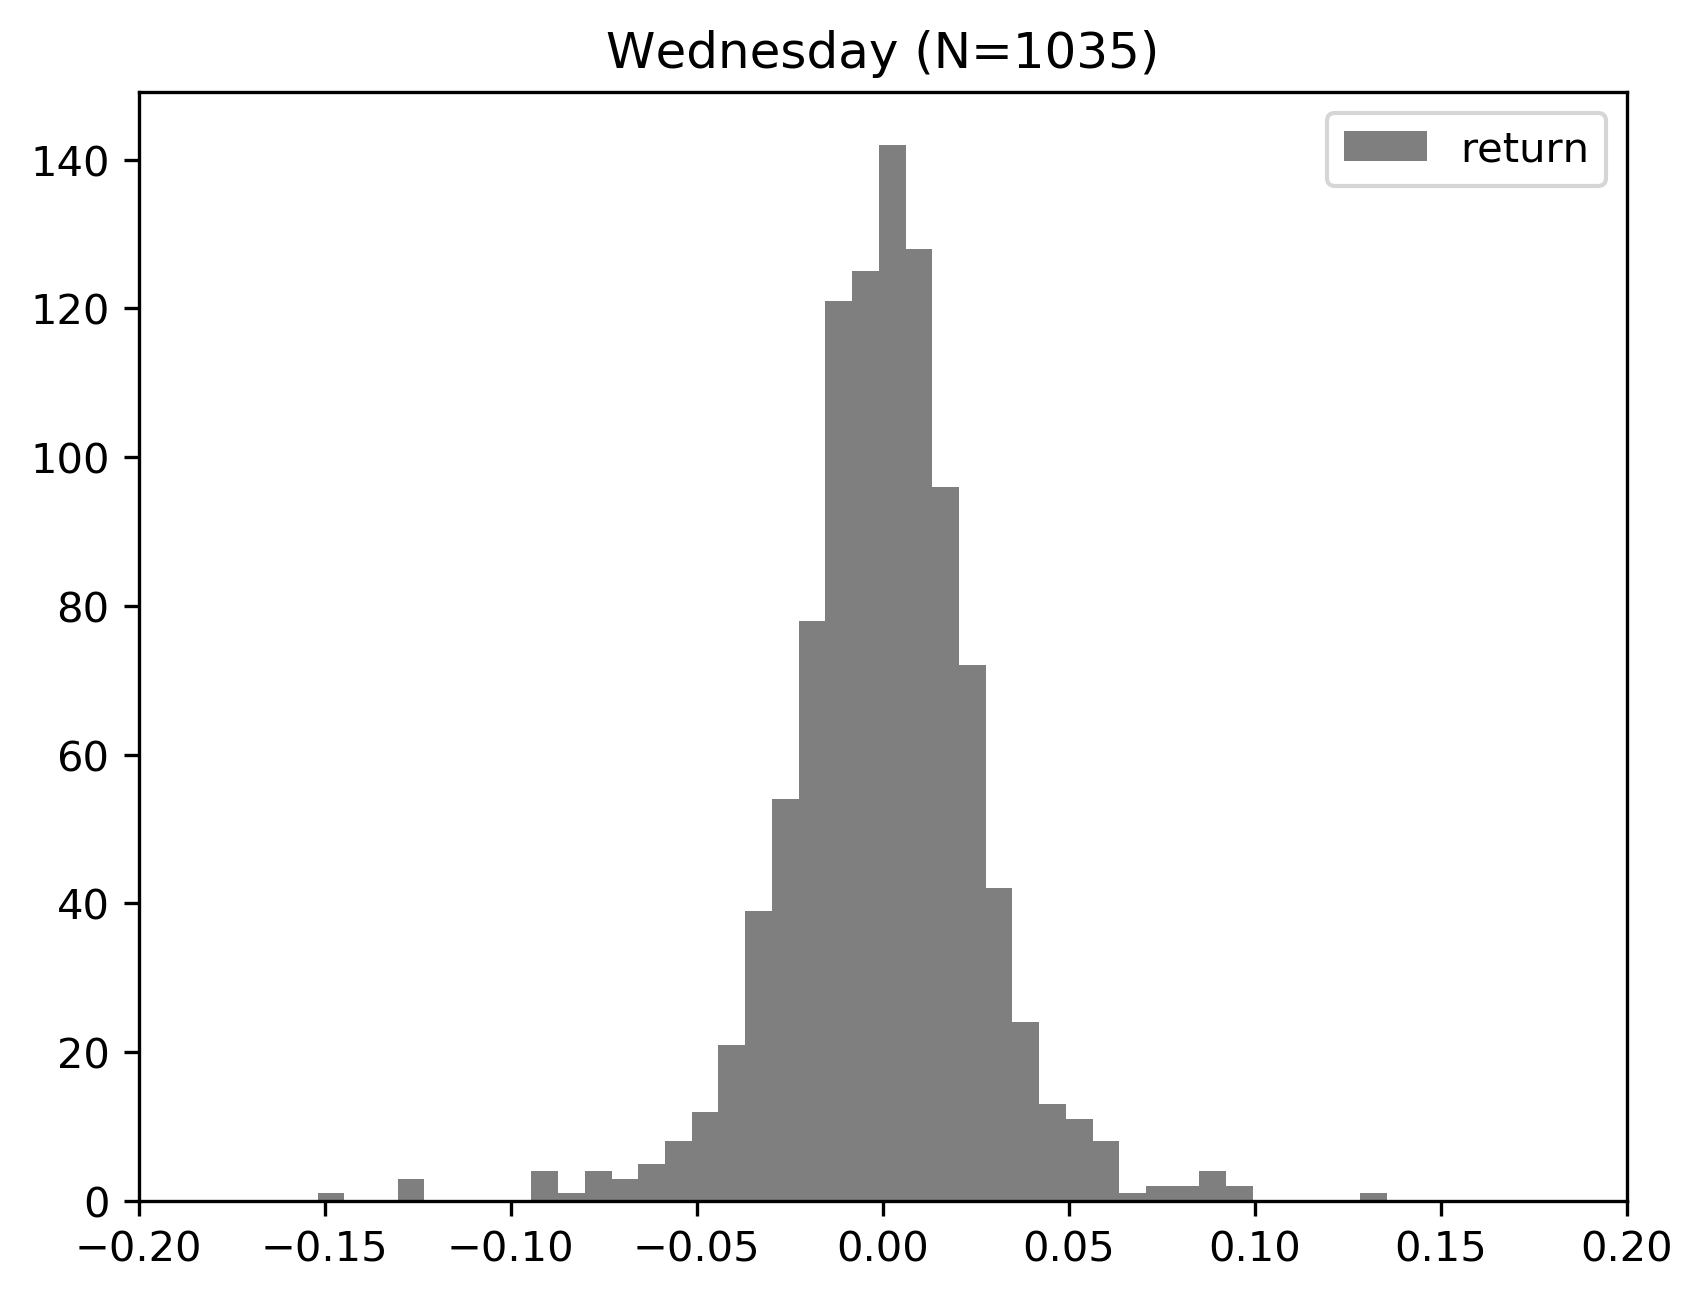
\includegraphics[width=0.45\linewidth]{figures/day_of_week_effect/dist_returns_Wednesday.png}
		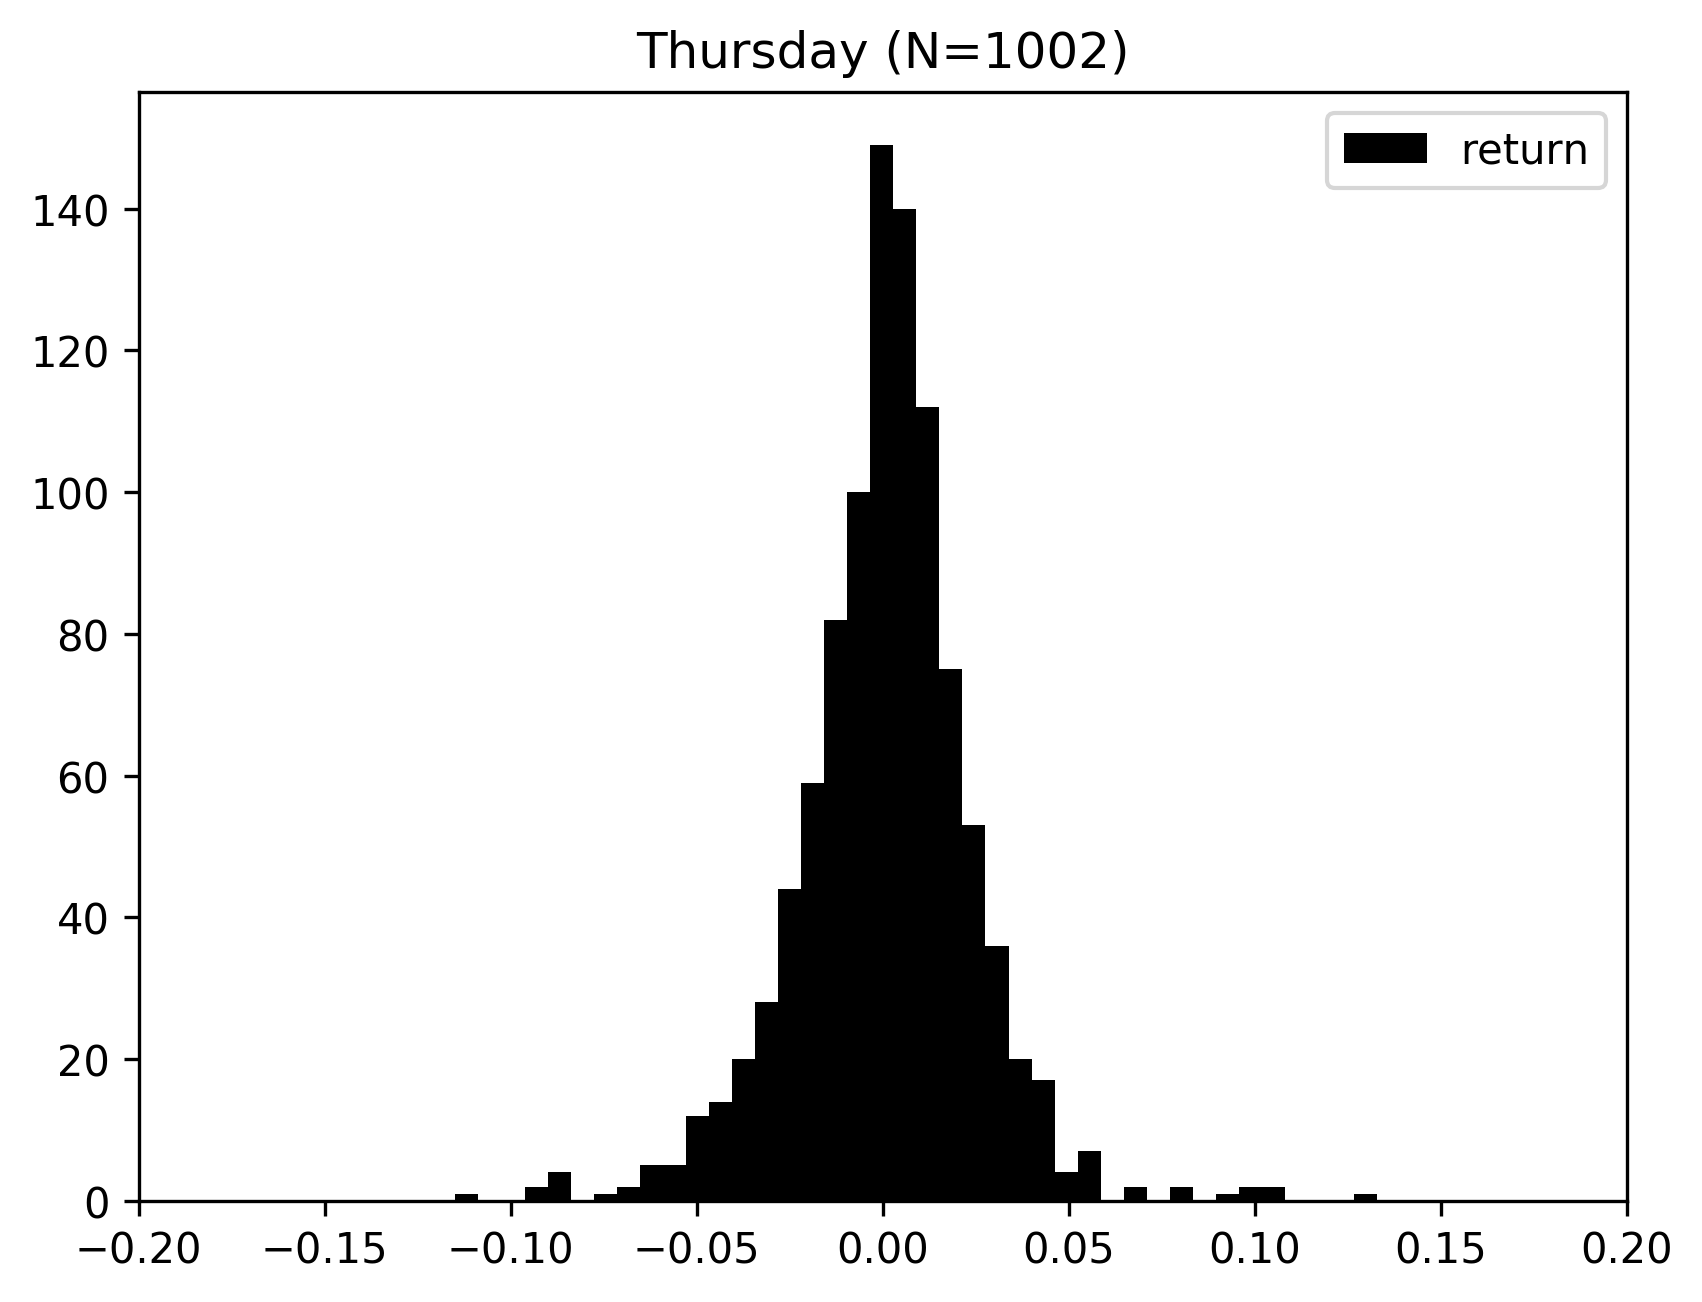
\includegraphics[width=0.45\linewidth]{figures/day_of_week_effect/dist_returns_Thursday.png}
		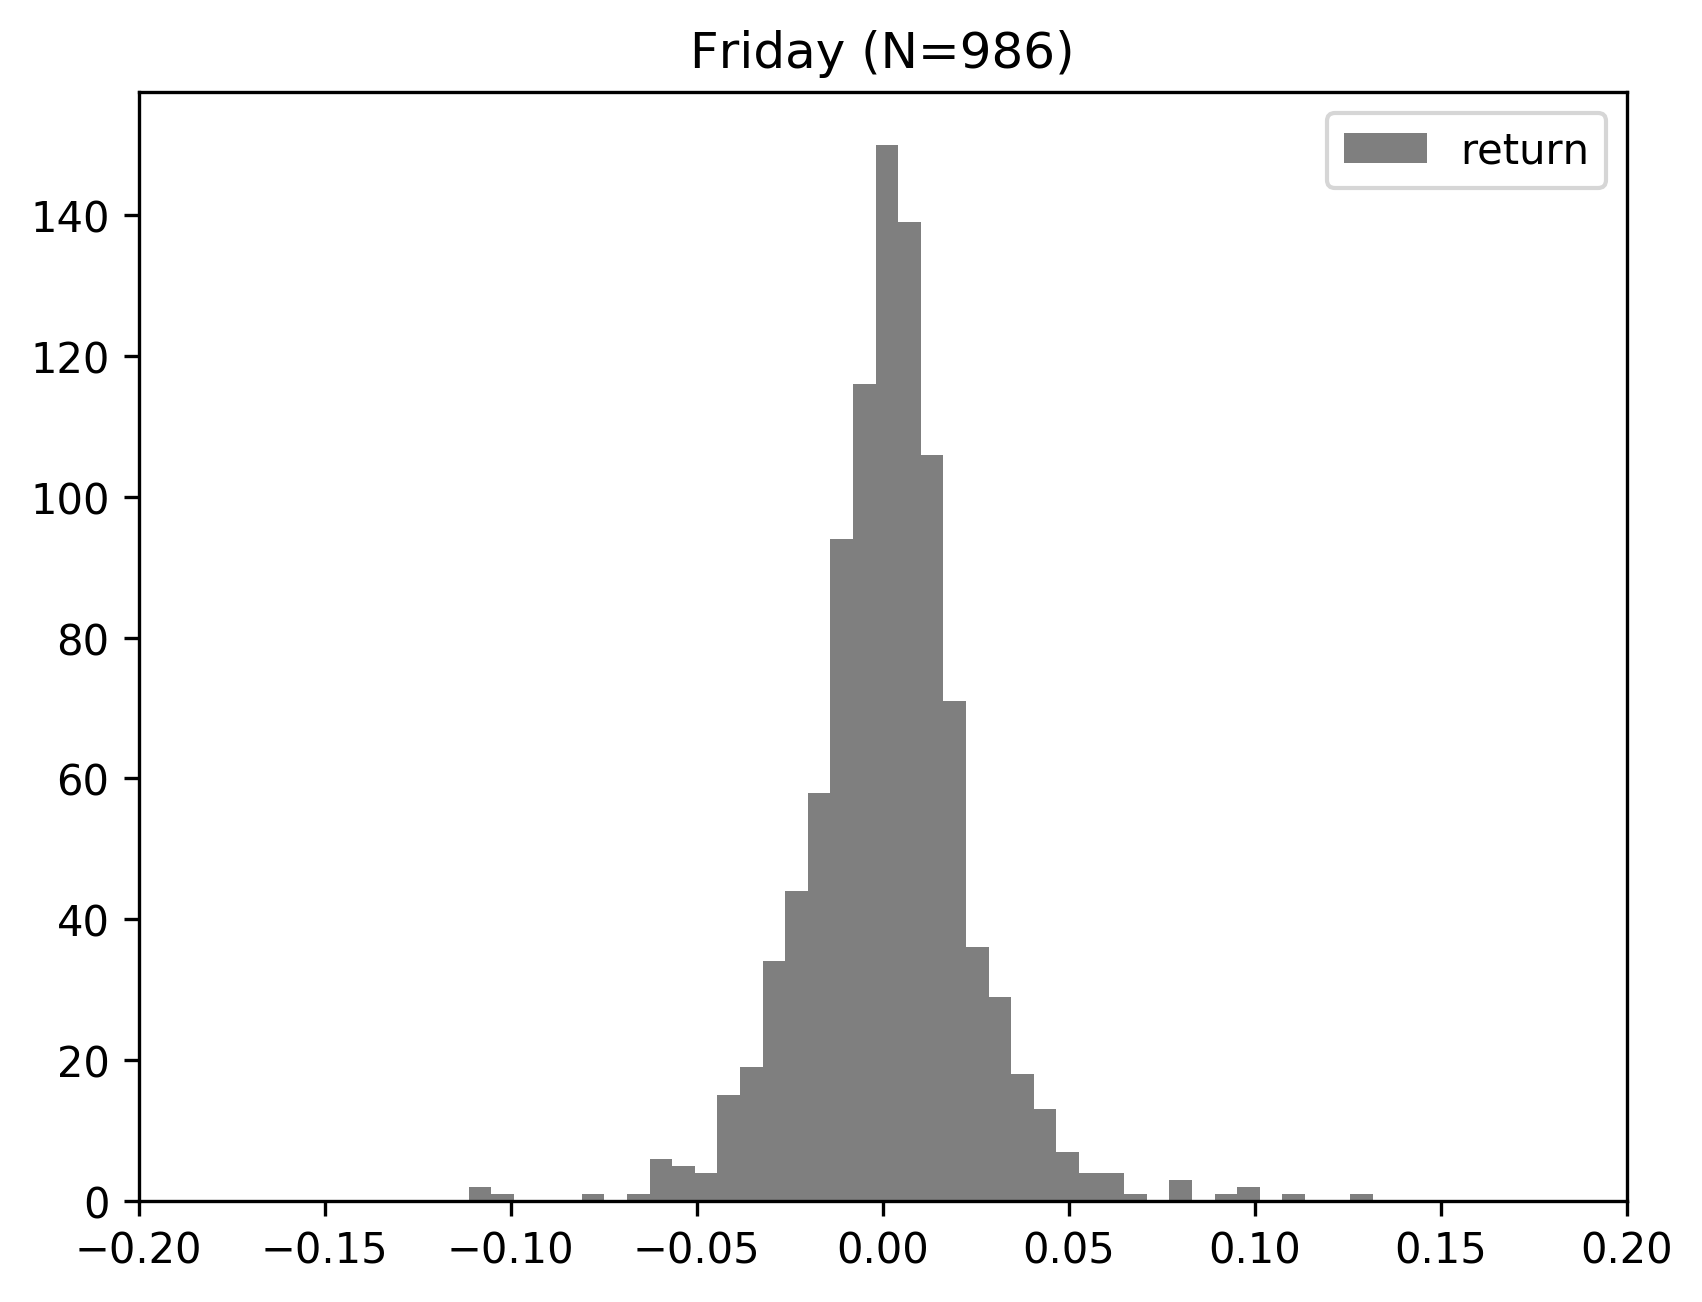
\includegraphics[width=0.45\linewidth]{figures/day_of_week_effect/dist_returns_Friday.png}
		\caption{Crude oil returns on each weekday. Weekend data are not available in the daily dataset provided by EIA. The range of y-axis in all five histograms are from -0.2 to 0.2. $N$s in parentheses denote the number of observations. See appendix for distributions of crude oil prices.}
	\end{figure}

	\par The \hl{two tables} below provide summary statistics for prices and returns on each day. It turns out that Monday is the only weekday with a mean return significantly less than zero.
	\begin{table}[H]
		\small
		\centering
		\begin{tabular}{l|c c c c}
			\toprule
			Day of the week & Num. Obs. & Mean & Std. & $3^{rd}$ Moment \\
			\midrule
			Monday & 927 & 62.072 & 26.493 & 7081.163 \\
			Tuesday & 1019 & 61.828 & 26.317 & 6895.638 \\
			Wednesday & 1022 & 61.810 & 26.398 & 7049.810 \\
			Thursday & 1002 & 62.005 & 26.431 & 6955.555 \\
			Friday & 986 & 62.079 & 26.247 & 6676.566 \\
			\midrule
			Total & 4956 & & & \\
			\bottomrule
		\end{tabular}
		\caption{Summary statistics of crude oil prices on each day of week}
	\end{table}

	\begin{table}[H]
		\small
		\centering
		\begin{tabular}{l|c c c c}
			\toprule
			Day of the week & Num. Obs. & Mean ($P$-Value) & Std. & $3^{rd}$ Moment \\
			\midrule
			Monday & 927 & \textbf{-0.002 (0.049)} & 0.025 & -0.0000019 \\
			Tuesday & 1018 & -0.000 (0.900) & 0.023 & -0.0000031 \\
			Wednesday & 1022 & 0.000 (0.884) & 0.027 & -0.0000054 \\
			Thursday & 1002 & 0.001 (0.361) & 0.024 & -0.0000006 \\
			Friday & 986 & \textbf{0.002 (0.0311)} & 0.023 & 0.0000021 \\
			\midrule
			Total & 4955 & & & \\
			\bottomrule
		\end{tabular}
		\caption{Summary statistics of crude oil returns on each day of week. The first day (January 1, 2000) of the oil price dataset was Saturday, and the observation on the following Monday (January 3) was missing. Hence, the return on Tuesday (January 4) could not be computed because it was the first trading day in this dataset, and there are only 1018 Tuesday in the dataset of returns. A value of $-0.000$ indicates a negative value with magnitude less than $0.0005$. $P$-values are calculated in a two-tailed $t$-test with $\mu_0 = 0$. Bold fonts indicate statistically significance at level $\alpha=0.05$.}
	\end{table}
	
	\subsubsection{Kolmogorov-Smirnov test for Distributional Similarities}
	\par Smirnov developed a non-parametric method of testing the equality between two continuous distributions, with CDFs $F(x)$ and $G(x)$ respectively, \cite{Smirnov1939}. Refer to Hodges' work for a detailed review on the Kolmogorov-Smirnov test \cite{Hodges1957}. I am using the two-tailed version of Kolmogorov-Smirnov test to check whether distributions of two different days are similar.
	Given two datasets, take returns on Monday and Tuesday for example, the null hypothesis says those two datasets are drawn from the same distribution, and the alternative says they are from different distributions \footnote{Different alternative hypotheses can be used in Kolmogorov–Smirnov test: i) $H_1: F(x) \geq G(x)$, ii) $H_1: F(x) \leq G(x)$, and iii) $H_1: F(x) \neq G(x)$. This paper is using the third (two-tailed) alternative hypothesis.}.
	Firstly, the Kolmogorov–Smirnov test constructs the empirical CDFs $F_{Mon, 927}(x)$ and $F_{Tue, 1018}(x)$ from the dataset. Then, the Kolmogorov–Smirnov statistic measures the maximum discrepancy between two distribution functions, which is
	\begin{align}
		D := \sup_x \abs{F_{Mon, 927}(x) - F_{Tue, 1018}(x)} \in [0, 1]
	\end{align}
	A smaller $D$-statistic implies stronger distributional similarity between two distributions. For instance, when $F_{Mon, 927}(x)$ and $F_{Tue, 1018}(x)$ are exactly the same, the $D$-statistic is zero. In contrast, let $X=0$ and $Y=1$ be two deterministic random variables, in this case, $D_{X, Y} = 1$.\\
	The test rejects $H_0$ at a significance level of $\alpha$ if 
	\begin{align}
		D > \sqrt{-\frac{1}{2} \ln \frac{\alpha}{2}} \sqrt{\frac{n+m}{nm}}
	\end{align}
	where $m$ and $n$ denote sizes of two datasets.
	\begin{table}[H]
		\small
		\centering
		\begin{tabular}{l|c|c|c|c|c}
			\toprule
			$D$-Statistic ($P$-Value)& Monday & Tuesday & Wednesday & Thursday & Friday \\
			\midrule
			Monday    & 0.000 (1.000) & \textbf{0.061 (0.048)} & \textbf{0.065 (0.030)} & \textbf{0.092 (0.001)} & \textbf{0.092 (0.001)} \\
			Tuesday   &               & 0.000 (1.000) & \textbf{0.044 (0.260)} & 0.036 (0.505) & 0.044 (0.264) \\
			Wednesday &               &               & 0.000 (1.000) & 0.053 (0.114) & \textbf{0.073 (0.009)} \\
			Thursday  &               &               &               & 0.000 (1.000) & 0.025 (0.900) \\
			Friday    &               &               &               &               & 0.000 (1.000) \\
			\bottomrule
		\end{tabular}
		\caption{The Kolmogorov-Smirnov $D$-Statistic for all pairs of distributions. Bold font indicates the null hypothesis is rejected at a significance level of 0.05, which implies discrepancy in distributions.}
	\end{table}
	\hl{The table above} presents the Kolmogorov-Smirnov $D$-Statistic for distributions of every pairs of days. At a significance level of 0.05, we can see that Monday follows a distribution significantly different from distributions other days follow. Because the dataset does not contain weekend data, the return on Monday is always computed using the difference between log prices on Monday and the previous Friday (Thursday if Friday is not a trading day and so on). Therefore, returns associated with Mondays pick the weekend effect. In fact, the distribution of returns on Monday (over weekend) is the only one with negative mean among distributions of all five days.

	\subsection{News and Sentiment Datasets}
	\paragraph{} The event sentiment dataset from RavenPack News Analytics (RPNA) tracks and analyzes all information of companies, organizations, countries, commodities, and currencies from Dow Jones Newswires, Wall Street Journal, Barron’s and MarketWatch ranges from January 1, 2000, to September 30, 2019. RavenPack records the exact date and time (measured using Coordinated Universal Time, UTC)  when each news is published. Because WTI crude oils are traded New York Mercantile Exchange, the UTC time is converted to Eastern Standard Time before further processing. Moreover, RPNA categorizes each event following the RavenPack taxonomy (figure: Ravenpack Event Taxonomy), which assigns a sequence of attributes describing each piece of news. In addition, for each event entry, using an algorithm combines results from surveying financial experts and pattern matching, RPNA assigns an Event Sentiment Score (ESS) between 0 and 100 to each event, measuring the short-term positive (100) and negative (0) financial or economic impact of this particular event. Refer to Appendix I for a complete list of attributes includes in this dataset.

	\par Focusing our attention on events about crude oil only, there are 106, 960 entries from the raw dataset left (around 15 events per day). In the figure below, panel A presents a distribution of ESS for all news related to crude oil in the time span of 20 years and panel B shows all distributions of events within each year.


	\subsection{Classifying News Type}
	
	\subsection{Case Studies of Events}
	\subsubsection{Positive Spike on November 30, 2016}
	\begin{figure}[H]
		\centering
		\small
		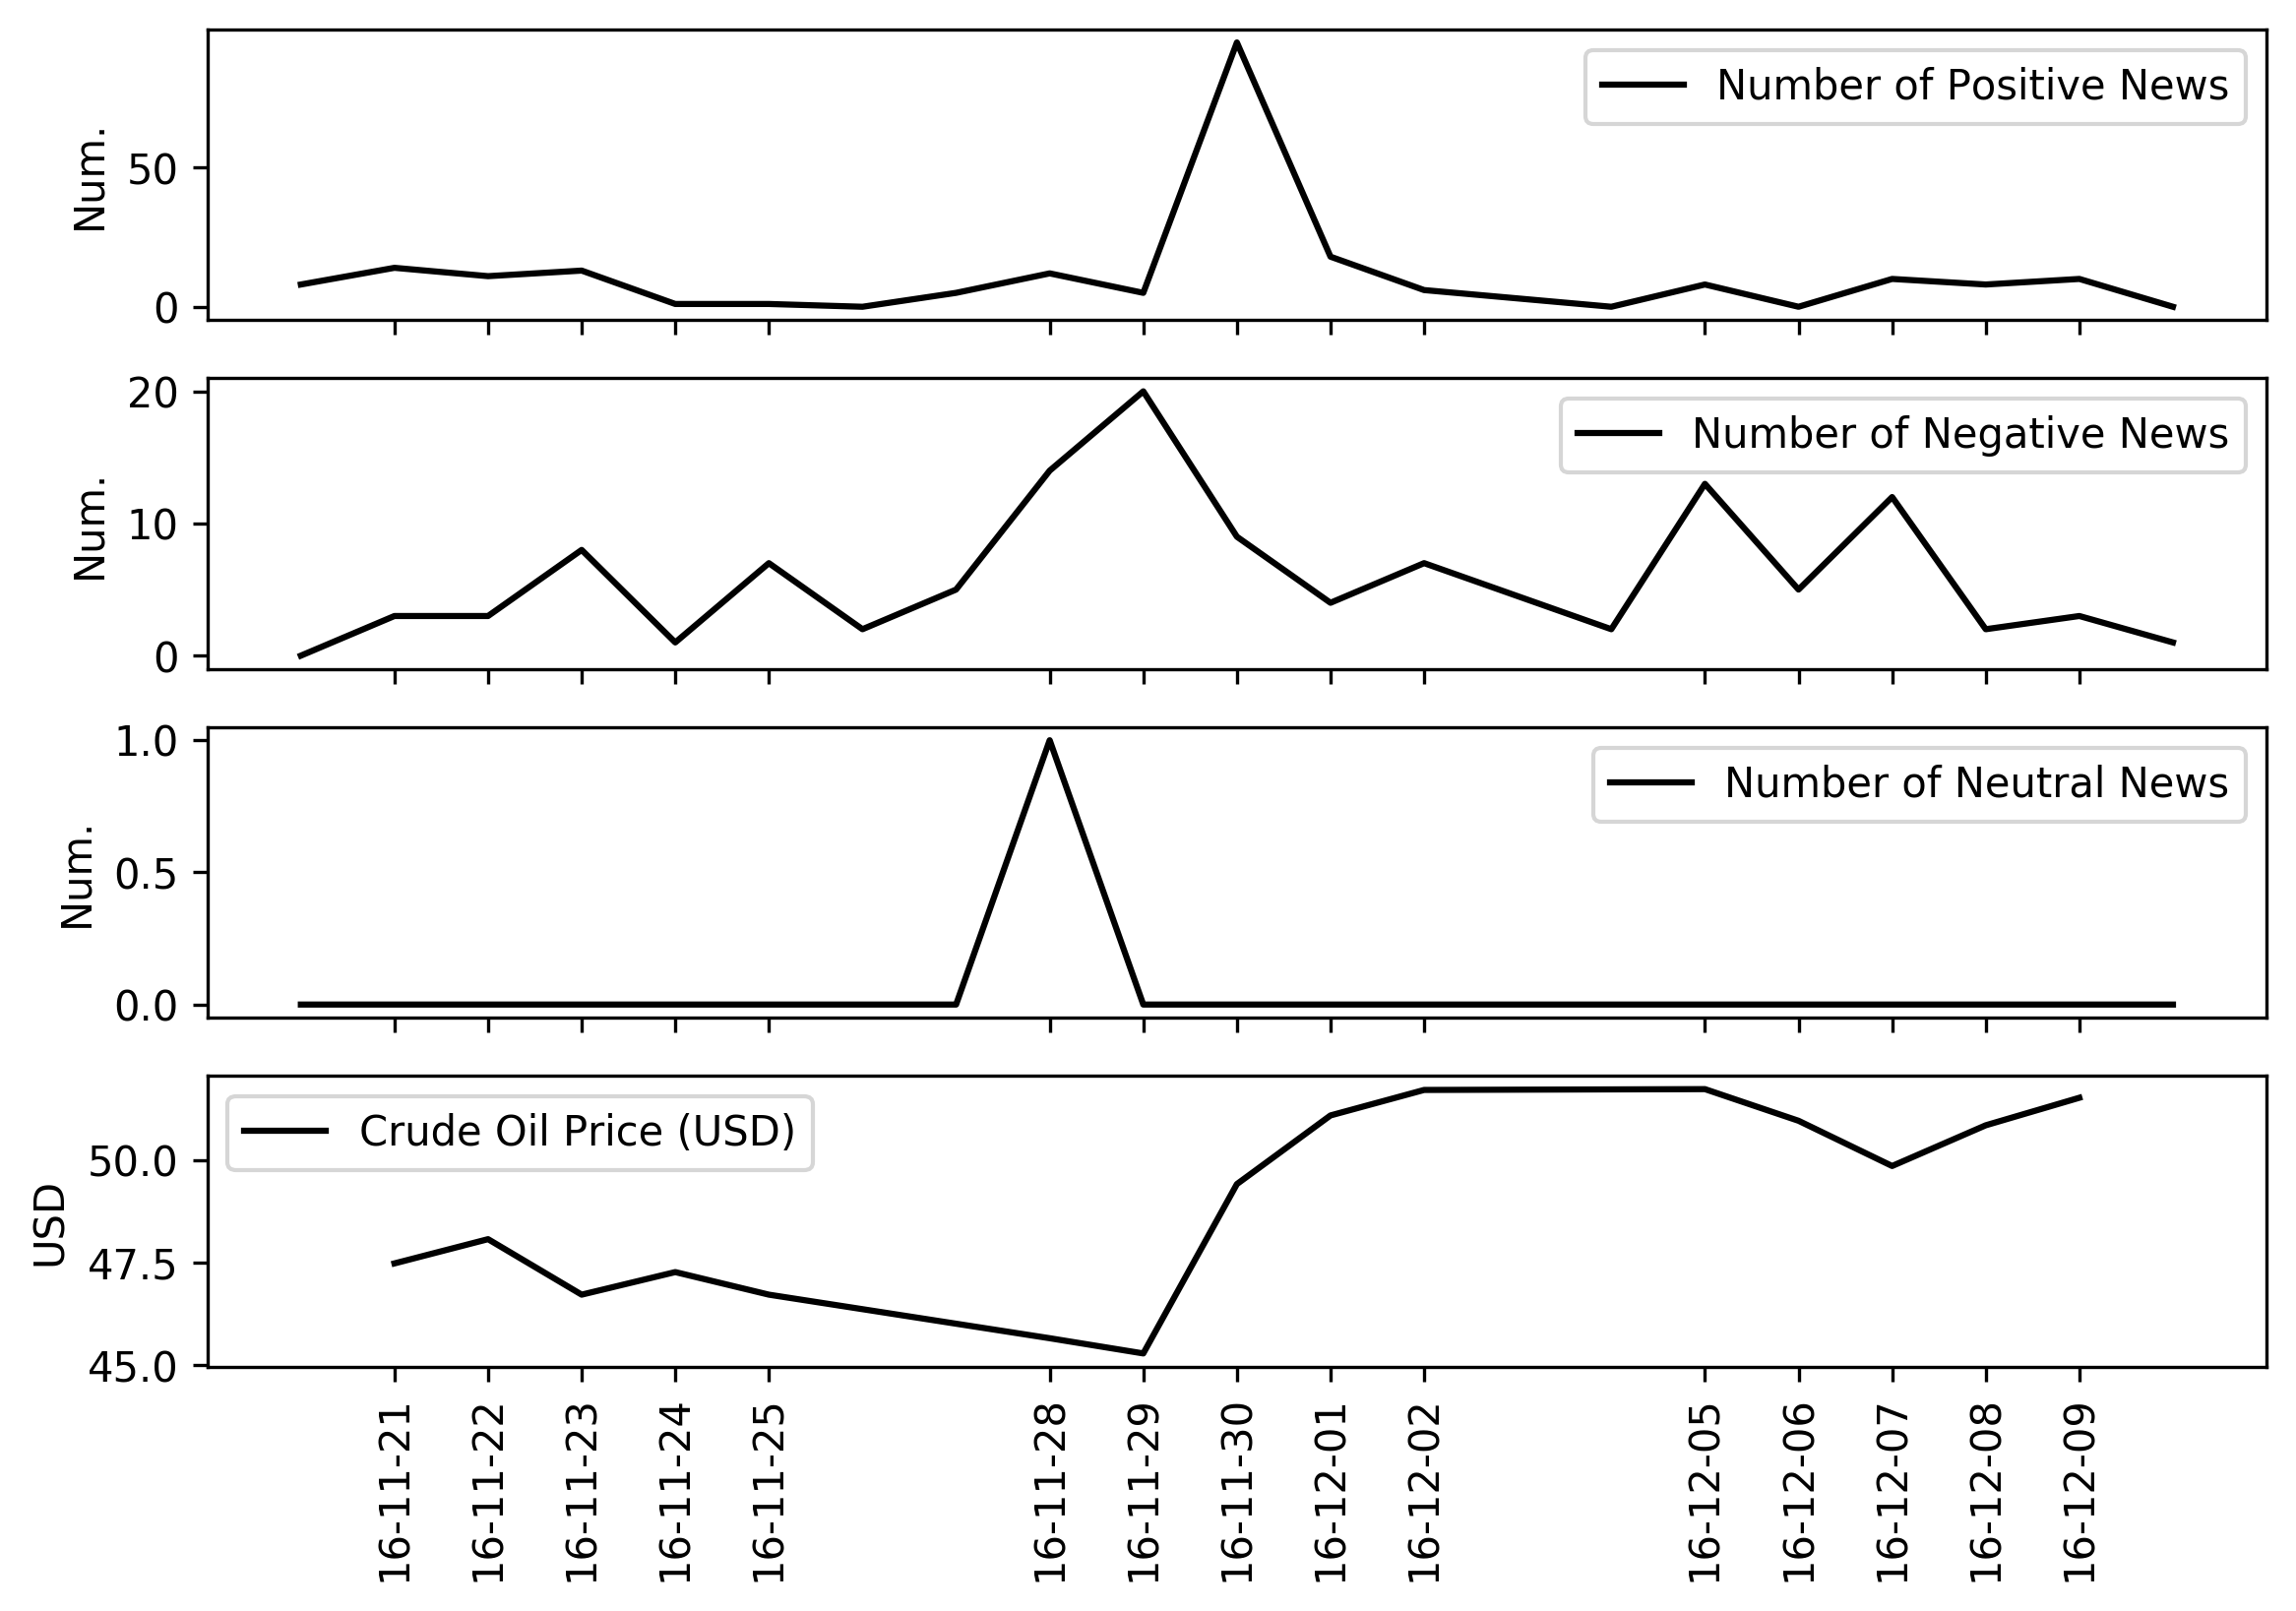
\includegraphics[width=\linewidth]{figures/case_studies/20161130_10d.png}
		\caption{}
	\end{figure}
	
	\subsubsection{Negative Spike on December 6, 2018}
	\begin{figure}[H]
		\centering
		\small
		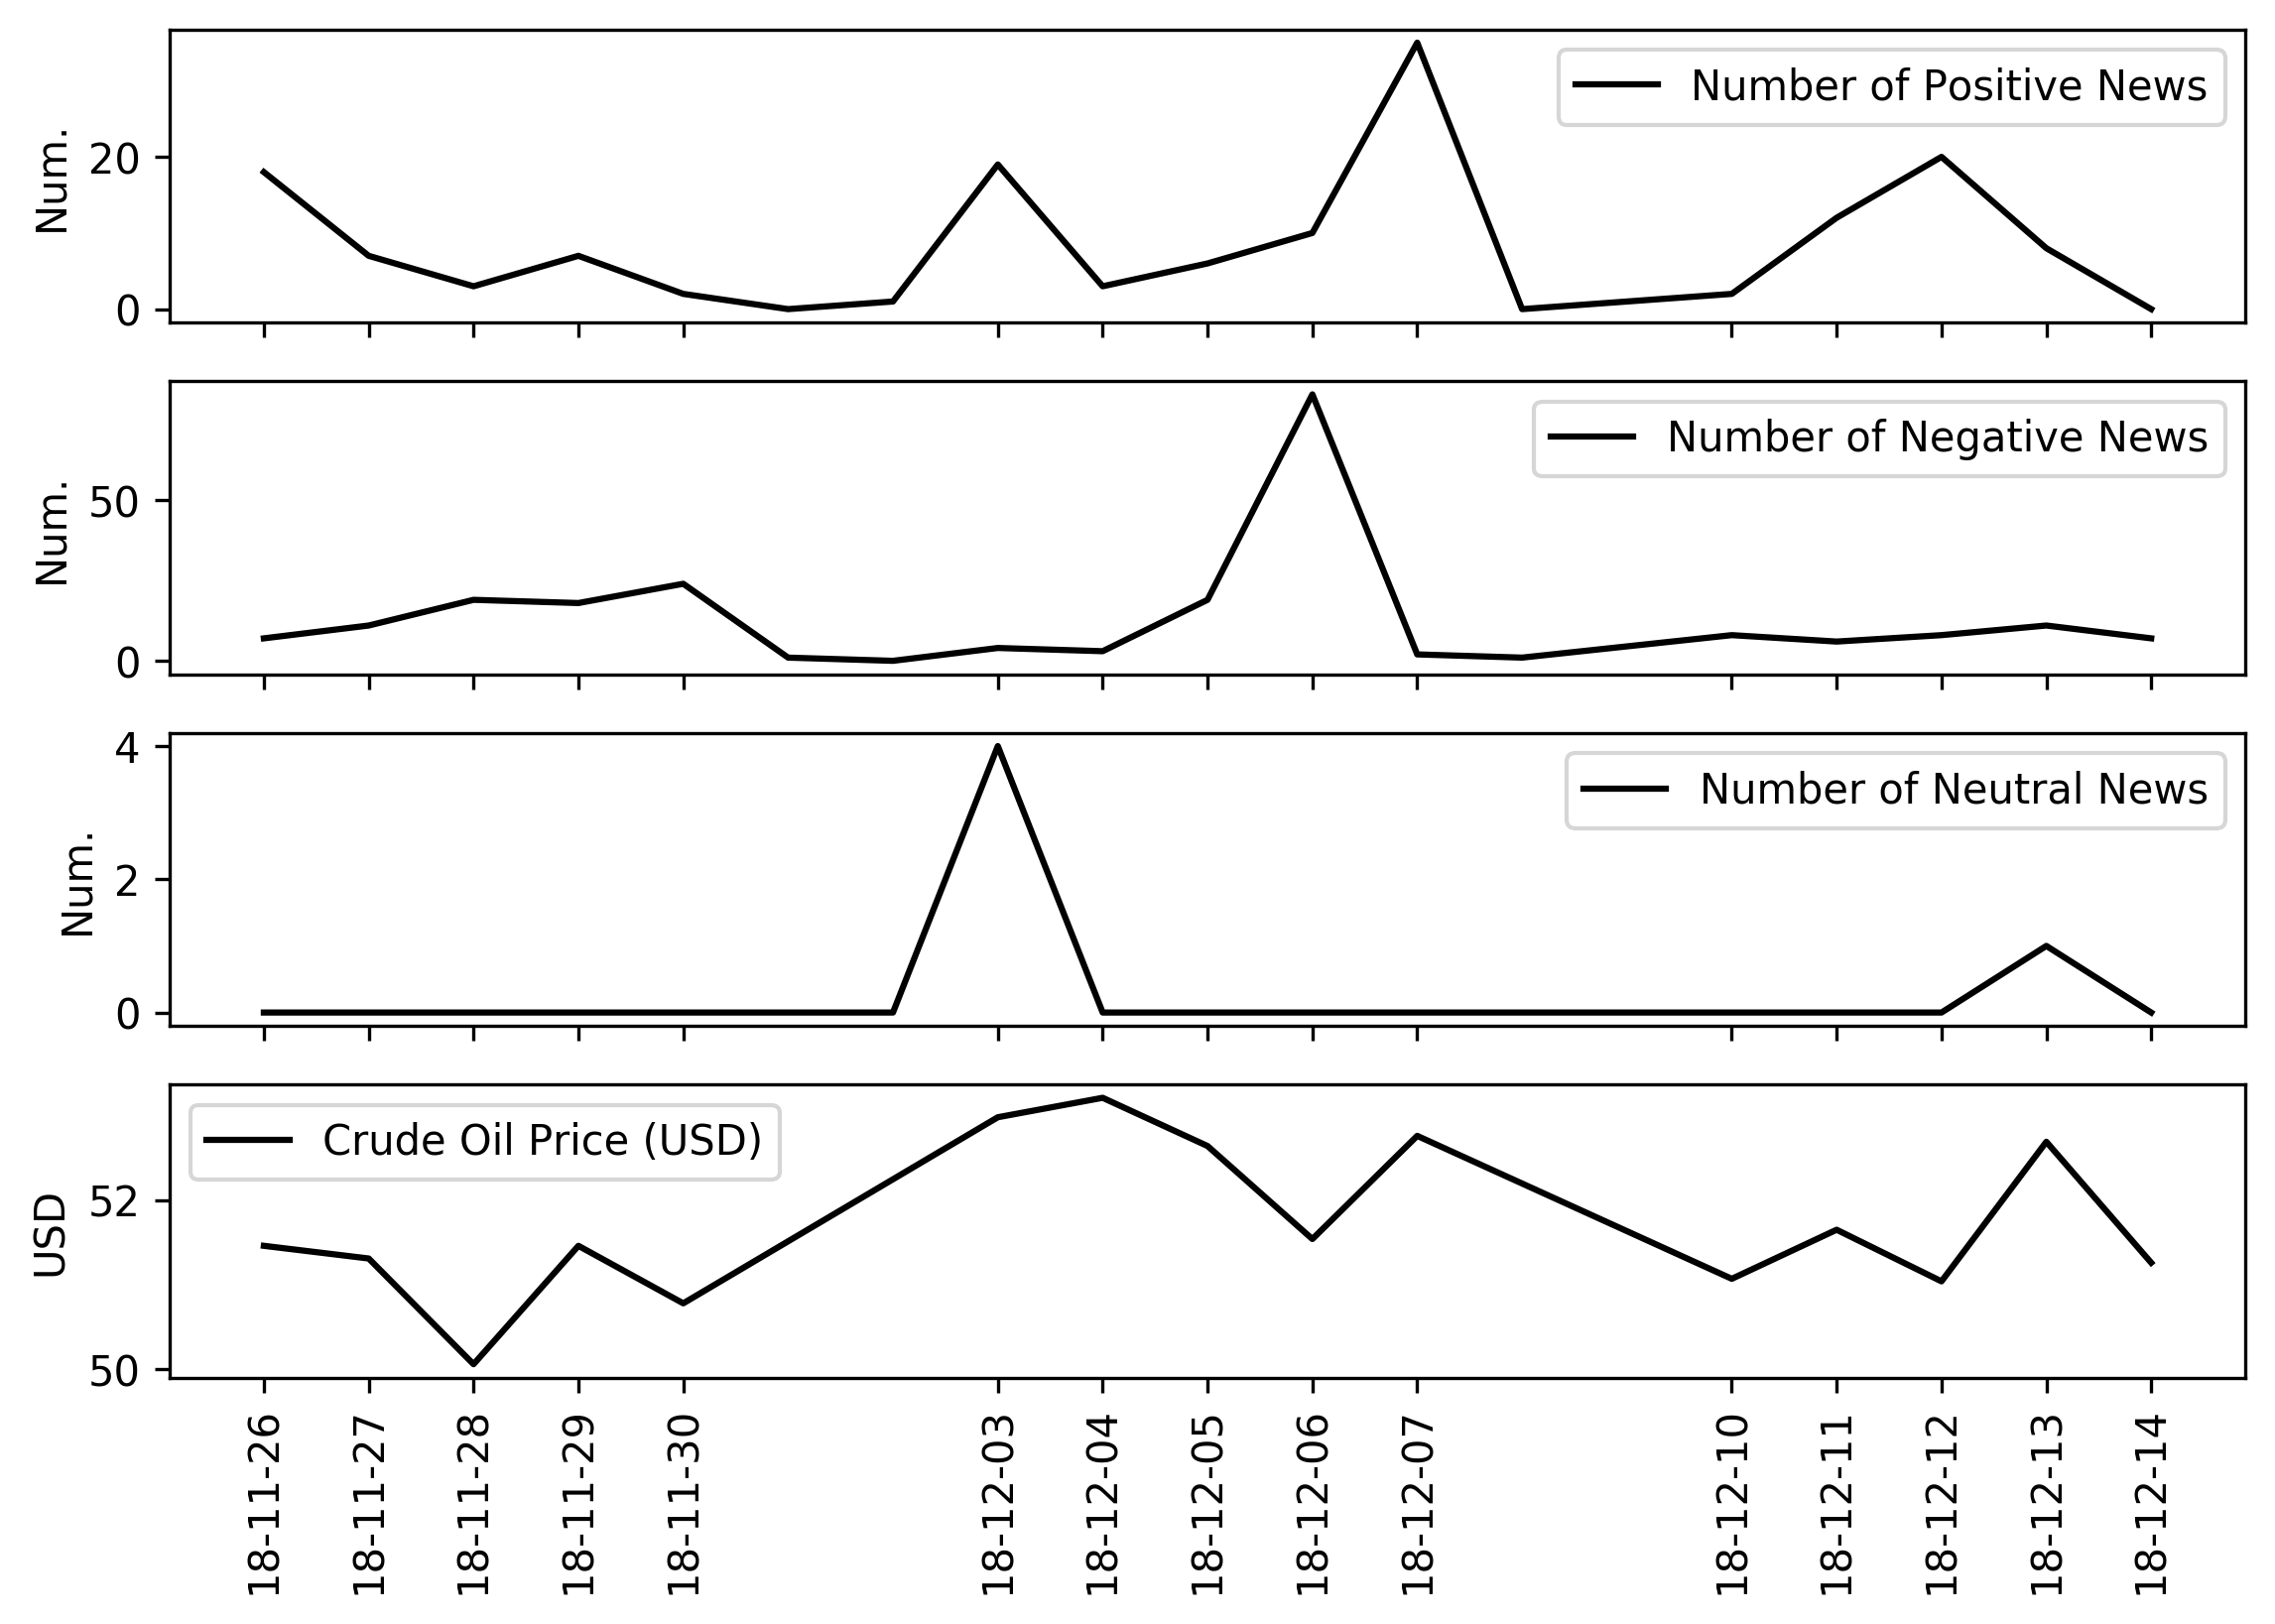
\includegraphics[width=\linewidth]{figures/case_studies/20181206_10d.png}
		\caption{}
	\end{figure}
	
	\subsubsection{Positive Spike on June. 12 - 13, 2019}
	\begin{figure}[H]
		\centering
		\small
		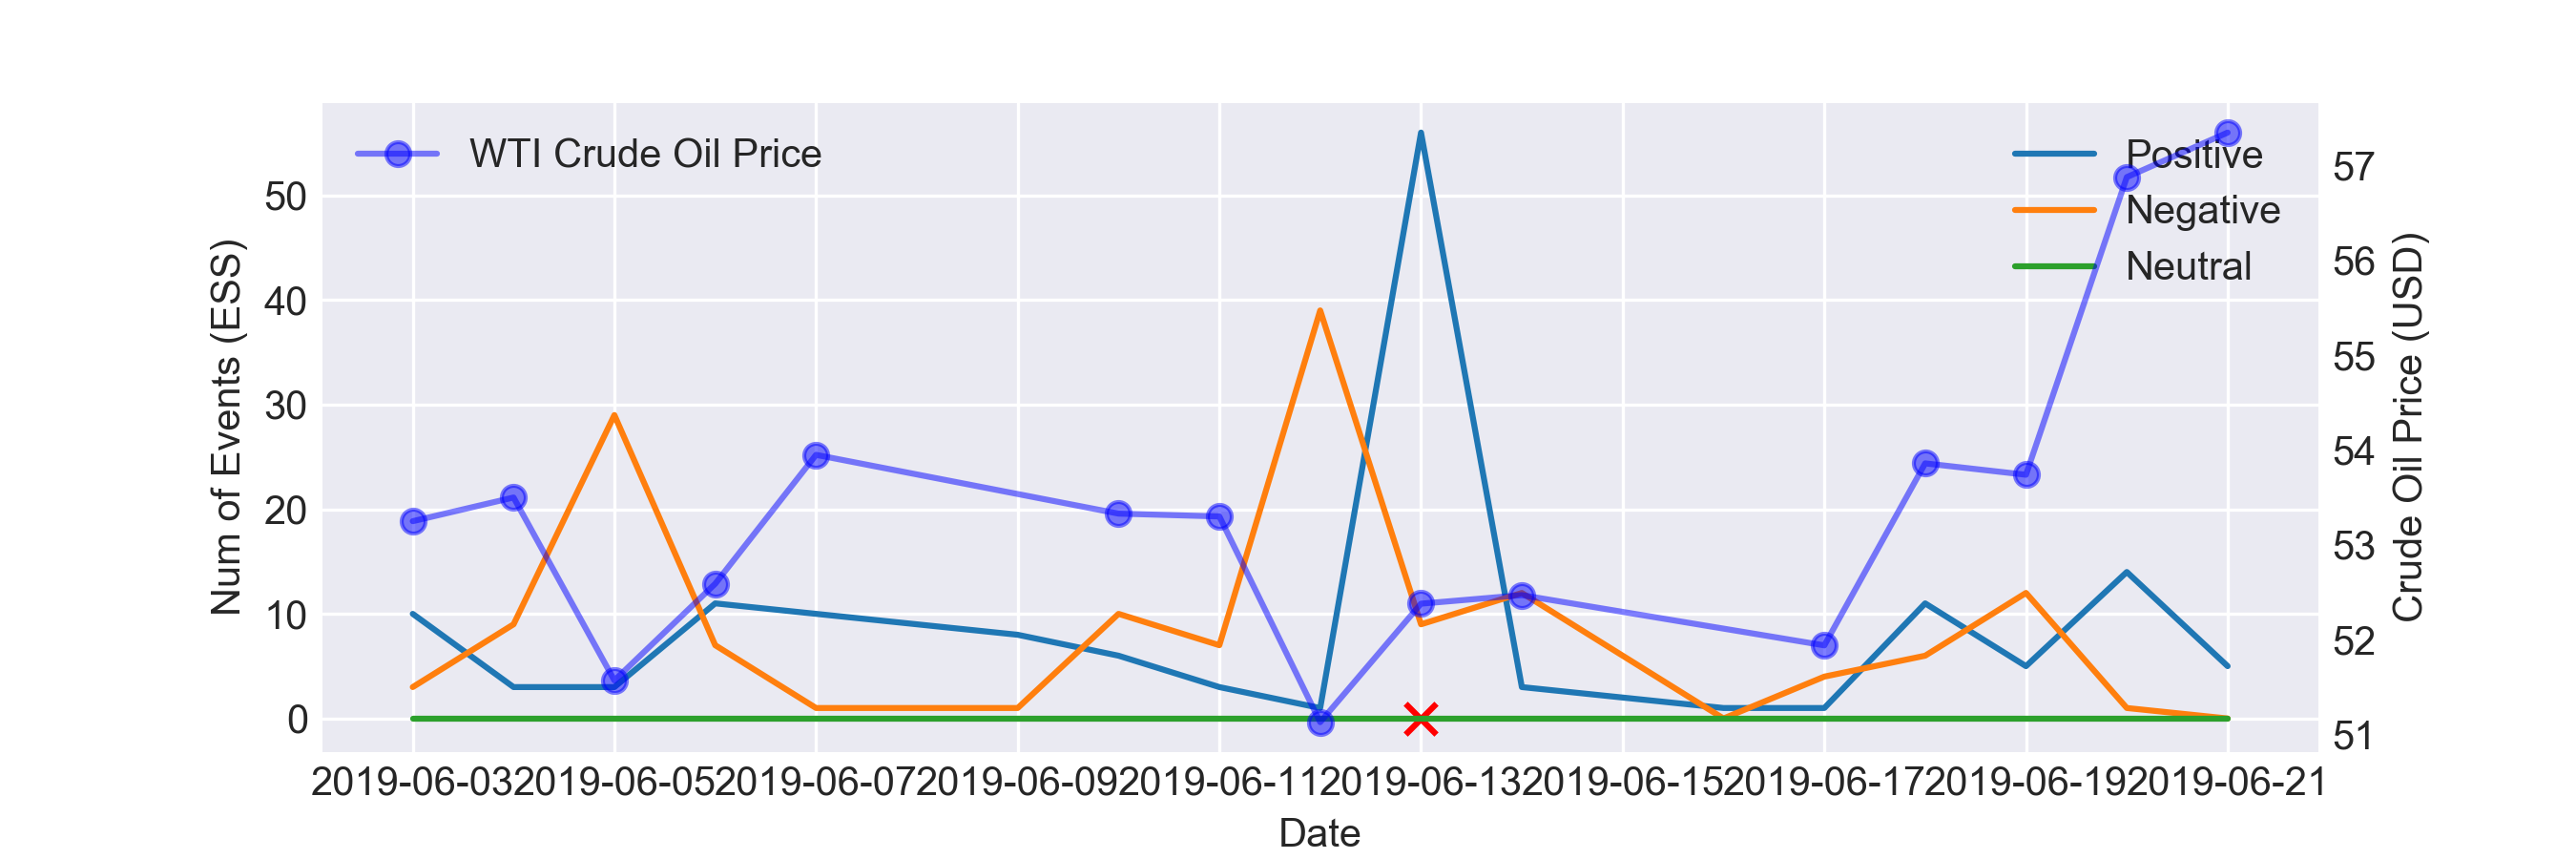
\includegraphics[width=\linewidth]{figures/case_studies/20190612_10d.png}
		\caption{}
	\end{figure}
	\section{Models}
	
	\section{Experiments}

	% Bib
	\bibliographystyle{apacite}
	
	\bibliography{thesis.bib}

	\section{Appendix: Supplementary Summary Statistics for Datasets}
	\begin{table}[H]
		\small
		\centering
		\begin{tabular}{l|c c c c c c c c c}
			\toprule
			Year & Num. Obs. & Mean & Median & Std. & Min & Max & ACF(1) & ACF(3) & ACF(5) \\
			\midrule
			2000 & 250 & 30.379 & 30.270 & 2.966 & 23.910 & 37.220 & 0.946 & 0.838 & 0.740 \\
			2001 & 250 & 25.983 & 27.185 & 3.560 & 17.500 & 32.210 & 0.973 & 0.924 & 0.880 \\
			2002 & 250 & 26.185 & 26.700 & 3.208 & 18.020 & 32.680 & 0.976 & 0.925 & 0.870 \\
			2003 & 250 & 31.075 & 30.770 & 2.624 & 25.250 & 37.960 & 0.943 & 0.864 & 0.764 \\
			2004 & 249 & 41.506 & 40.700 & 5.775 & 32.490 & 56.370 & 0.982 & 0.949 & 0.915 \\
			2005 & 251 & 56.637 & 57.330 & 6.252 & 42.160 & 69.910 & 0.969 & 0.917 & 0.876 \\
			2006 & 249 & 66.055 & 65.650 & 5.586 & 55.900 & 77.050 & 0.975 & 0.929 & 0.893 \\
			2007 & 252 & 72.341 & 69.735 & 12.853 & 50.510 & 99.160 & 0.986 & 0.956 & 0.924 \\
			2008 & 253 & 99.672 & 104.830 & 28.563 & 30.280 & 145.310 & 0.986 & 0.958 & 0.926 \\
			2009 & 252 & 61.950 & 67.025 & 13.361 & 34.030 & 81.030 & 0.985 & 0.959 & 0.928 \\
			2010 & 252 & 79.476 & 79.735 & 5.242 & 64.780 & 91.480 & 0.953 & 0.853 & 0.759 \\
			2011 & 252 & 94.881 & 95.790 & 8.063 & 75.400 & 113.390 & 0.968 & 0.900 & 0.828 \\
			2012 & 252 & 94.053 & 92.605 & 7.713 & 77.720 & 109.390 & 0.979 & 0.946 & 0.914 \\
			2013 & 252 & 97.983 & 96.325 & 5.451 & 86.650 & 110.620 & 0.977 & 0.927 & 0.881 \\
			2014 & 252 & 93.172 & 97.850 & 13.519 & 53.450 & 107.950 & 0.978 & 0.936 & 0.895 \\
			2015 & 252 & 48.657 & 47.870 & 6.814 & 34.550 & 61.360 & 0.972 & 0.928 & 0.888 \\
			2016 & 252 & 43.294 & 45.080 & 6.727 & 26.190 & 54.010 & 0.978 & 0.932 & 0.893 \\
			2017 & 250 & 50.800 & 50.385 & 3.914 & 42.480 & 60.460 & 0.968 & 0.905 & 0.846 \\
			2018 & 249 & 65.227 & 66.380 & 6.517 & 44.480 & 77.410 & 0.961 & 0.888 & 0.812 \\
			2019 & 187 & 57.037 & 56.580 & 3.986 & 46.310 & 66.240 & 0.924 & 0.811 & 0.732 \\
			\midrule
			Total & 4956 & 61.956 & 58.915 & 26.376 & 17.500 & 145.310 & 0.998 & 0.995 & 0.992 \\
			\bottomrule
		\end{tabular}
		\caption{Summary Statistics for Crude Oil Prices. Note that this dataset only include nine months of 2019.}
	\end{table}
	
	\begin{figure}[H]
		\centering
		\small
		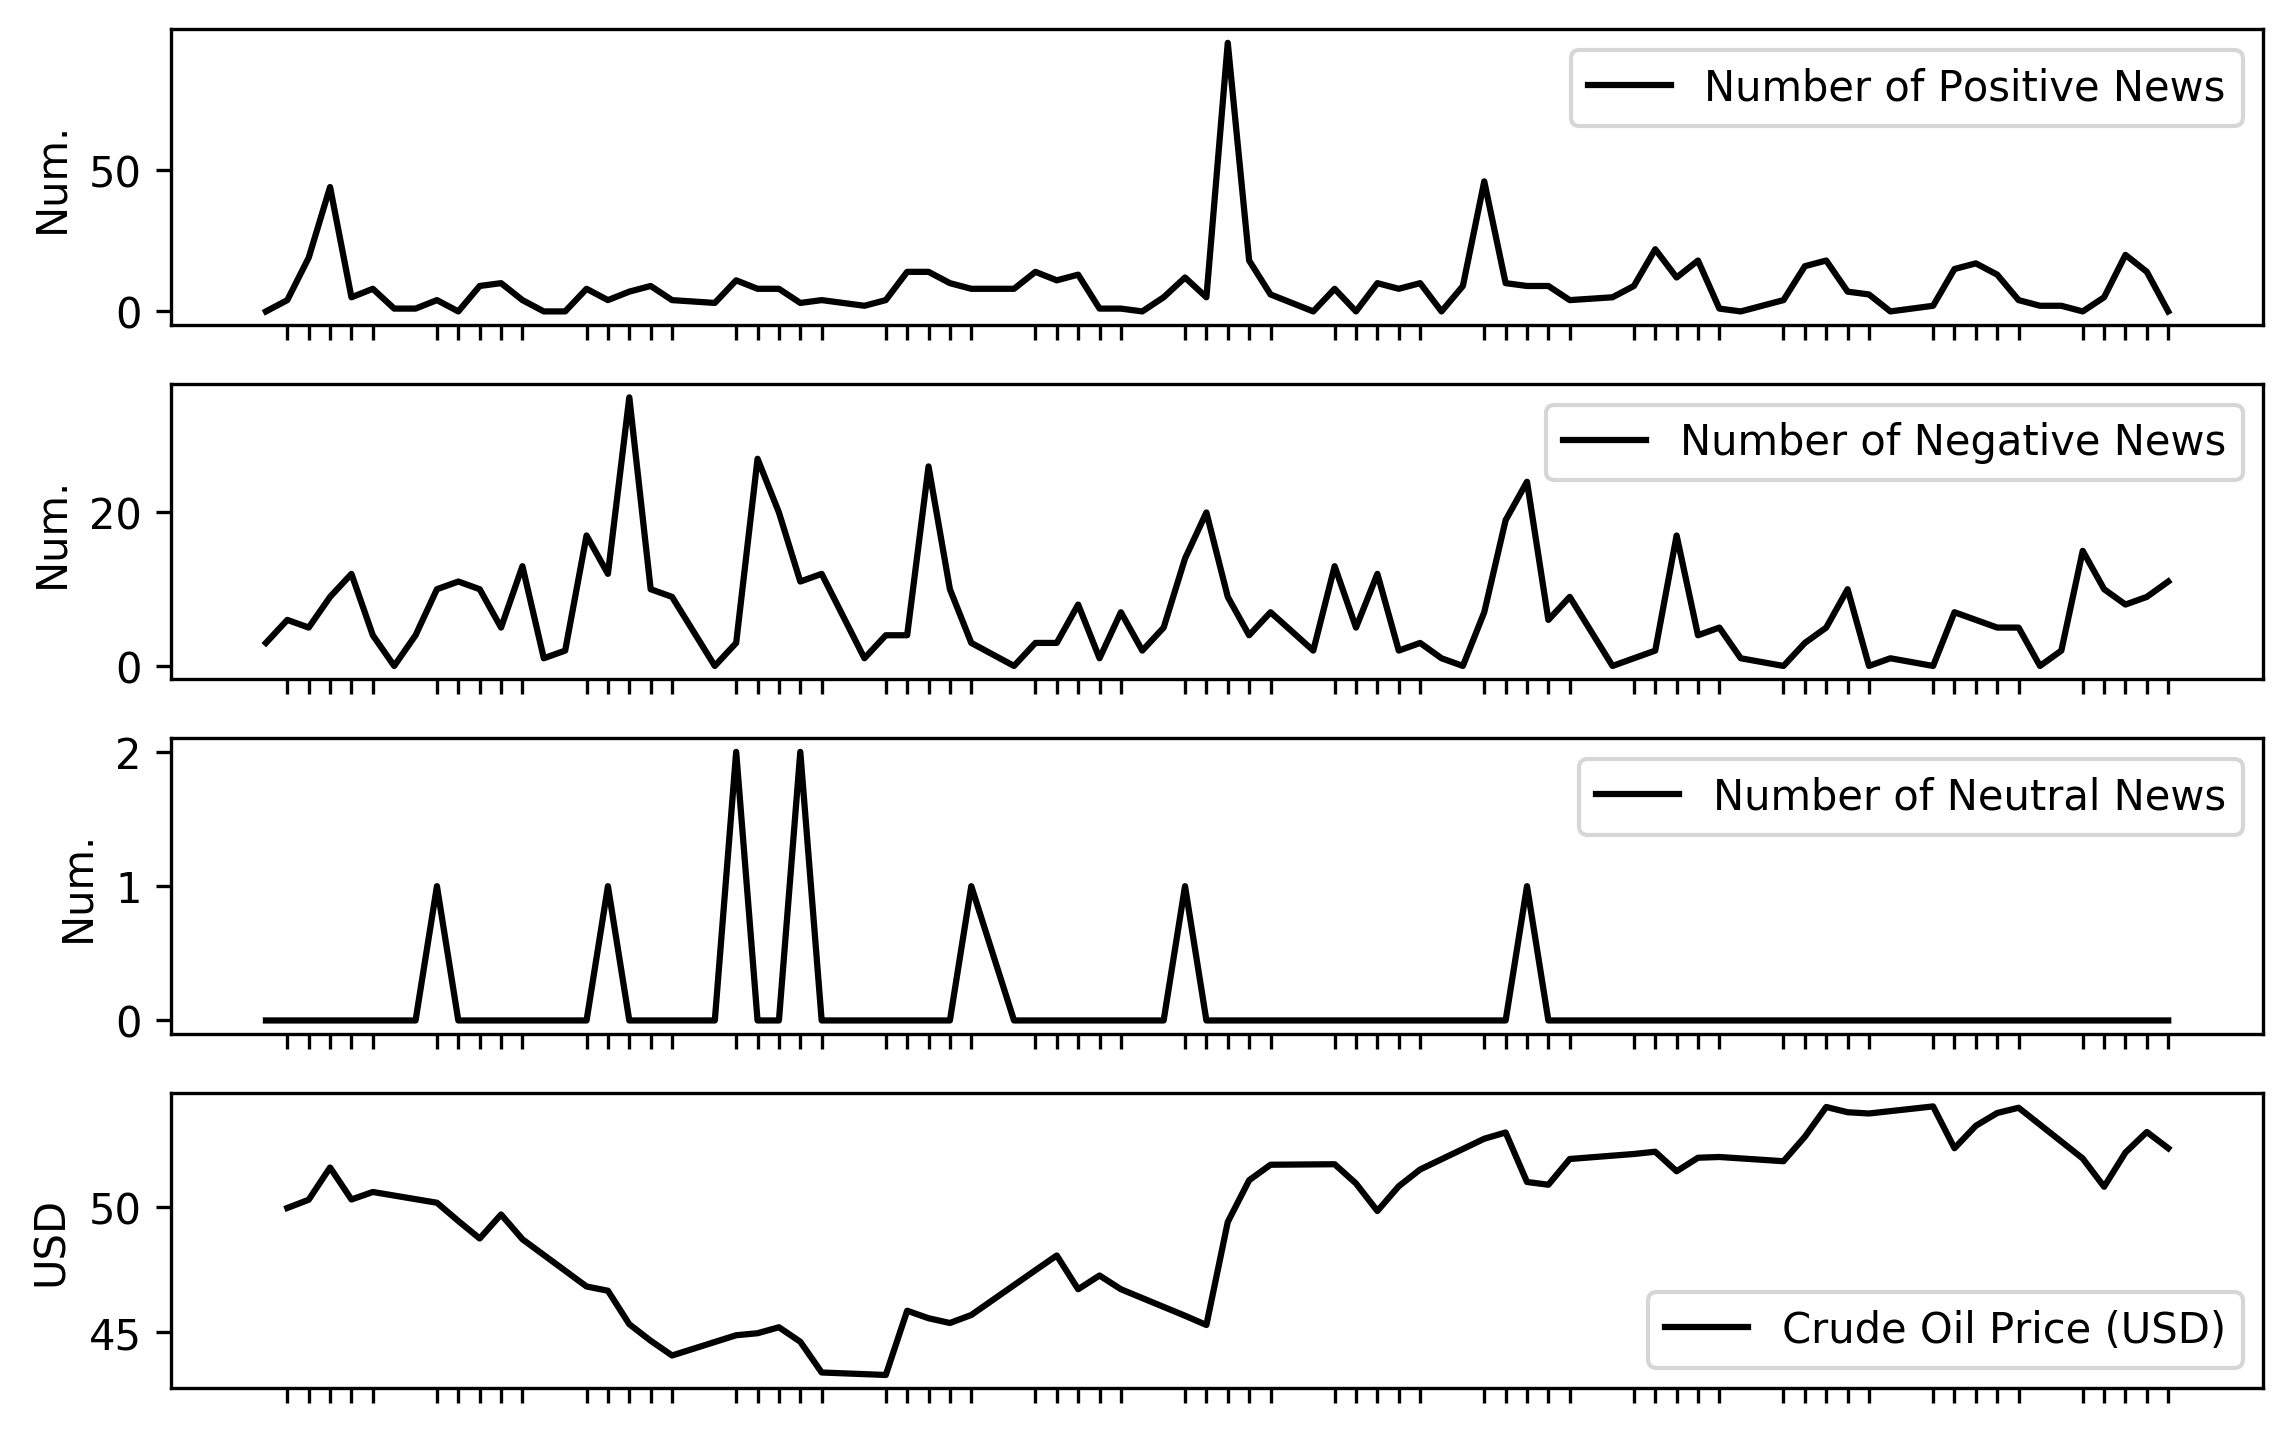
\includegraphics[width=\linewidth]{figures/case_studies/20161130_45d.png}
		\caption{}
	\end{figure}
	\begin{figure}[H]
		\centering
		\small
		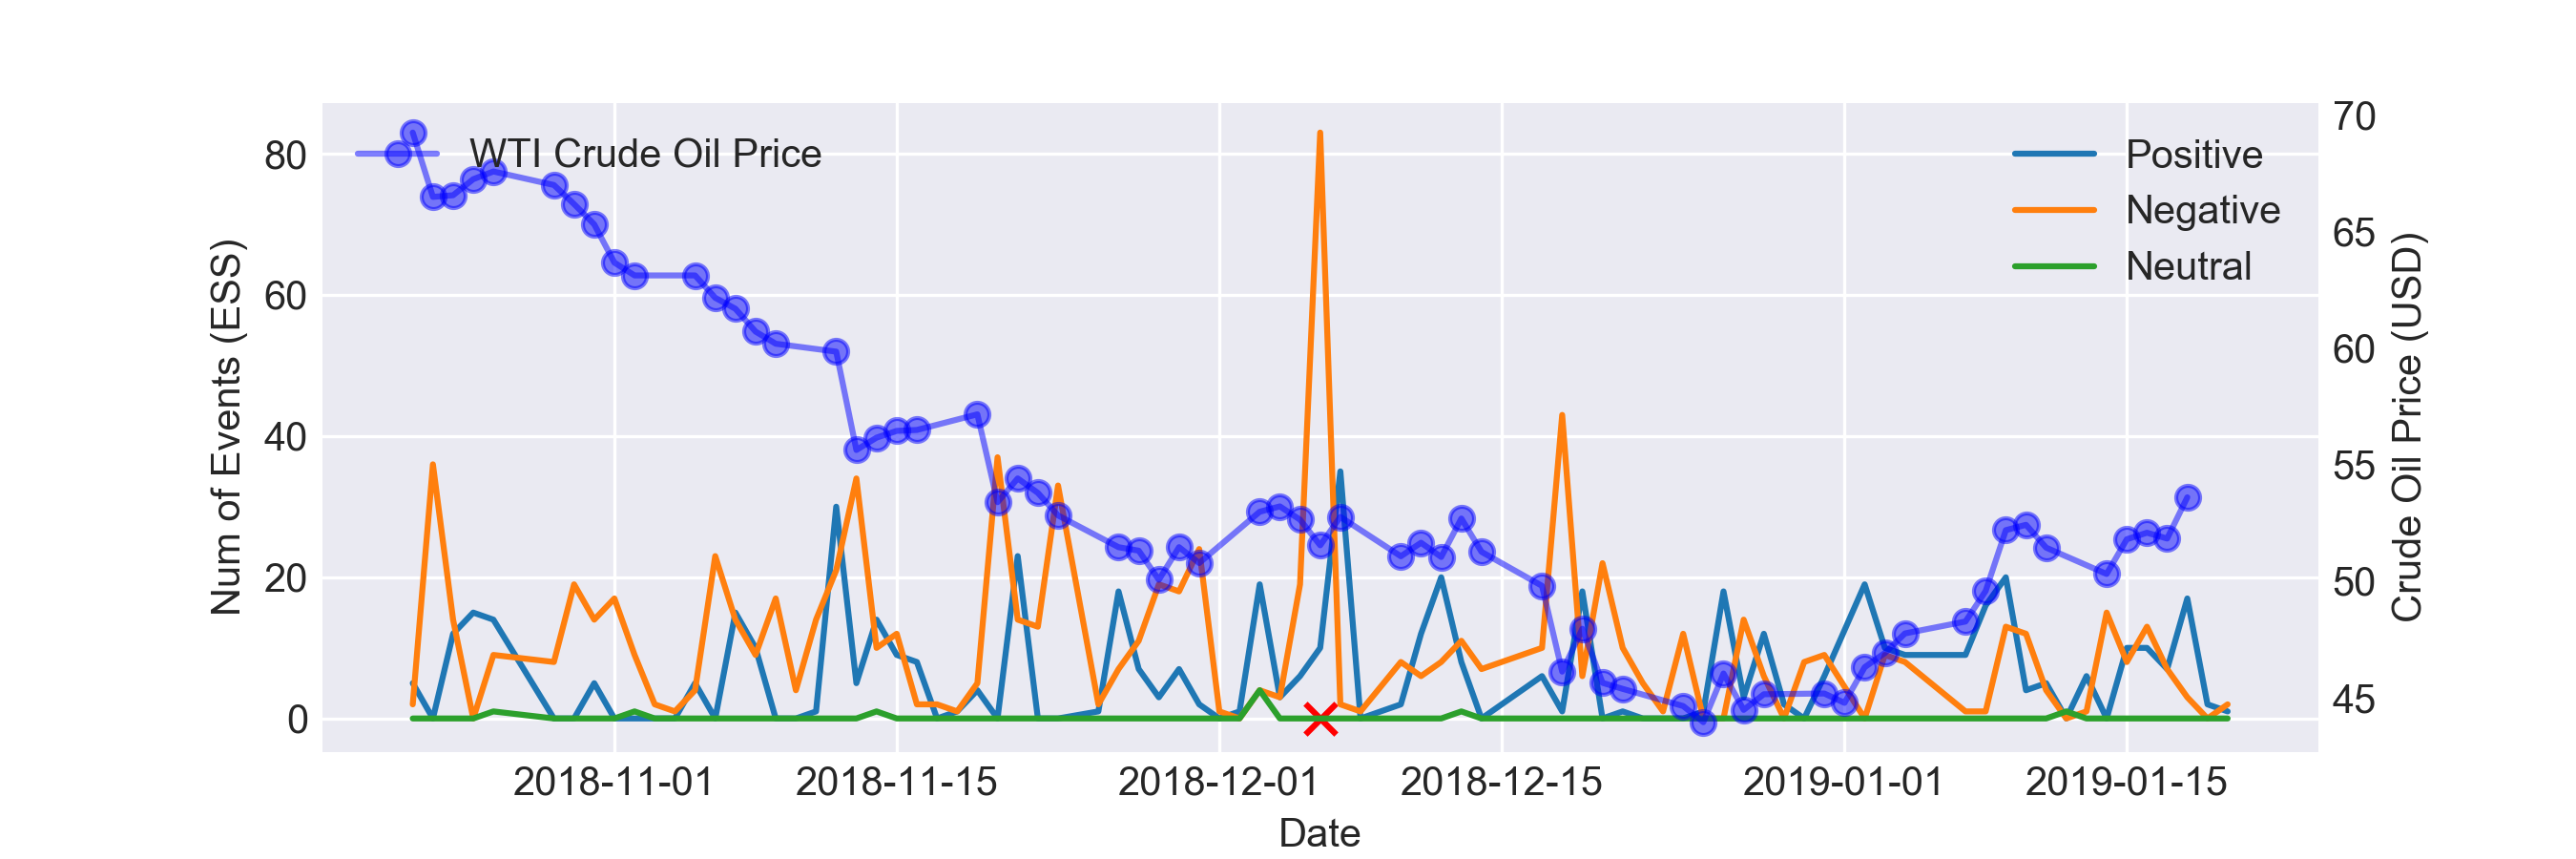
\includegraphics[width=\linewidth]{figures/case_studies/20181206_45d.png}
		\caption{}
	\end{figure}
	\begin{figure}[H]
		\centering
		\small
		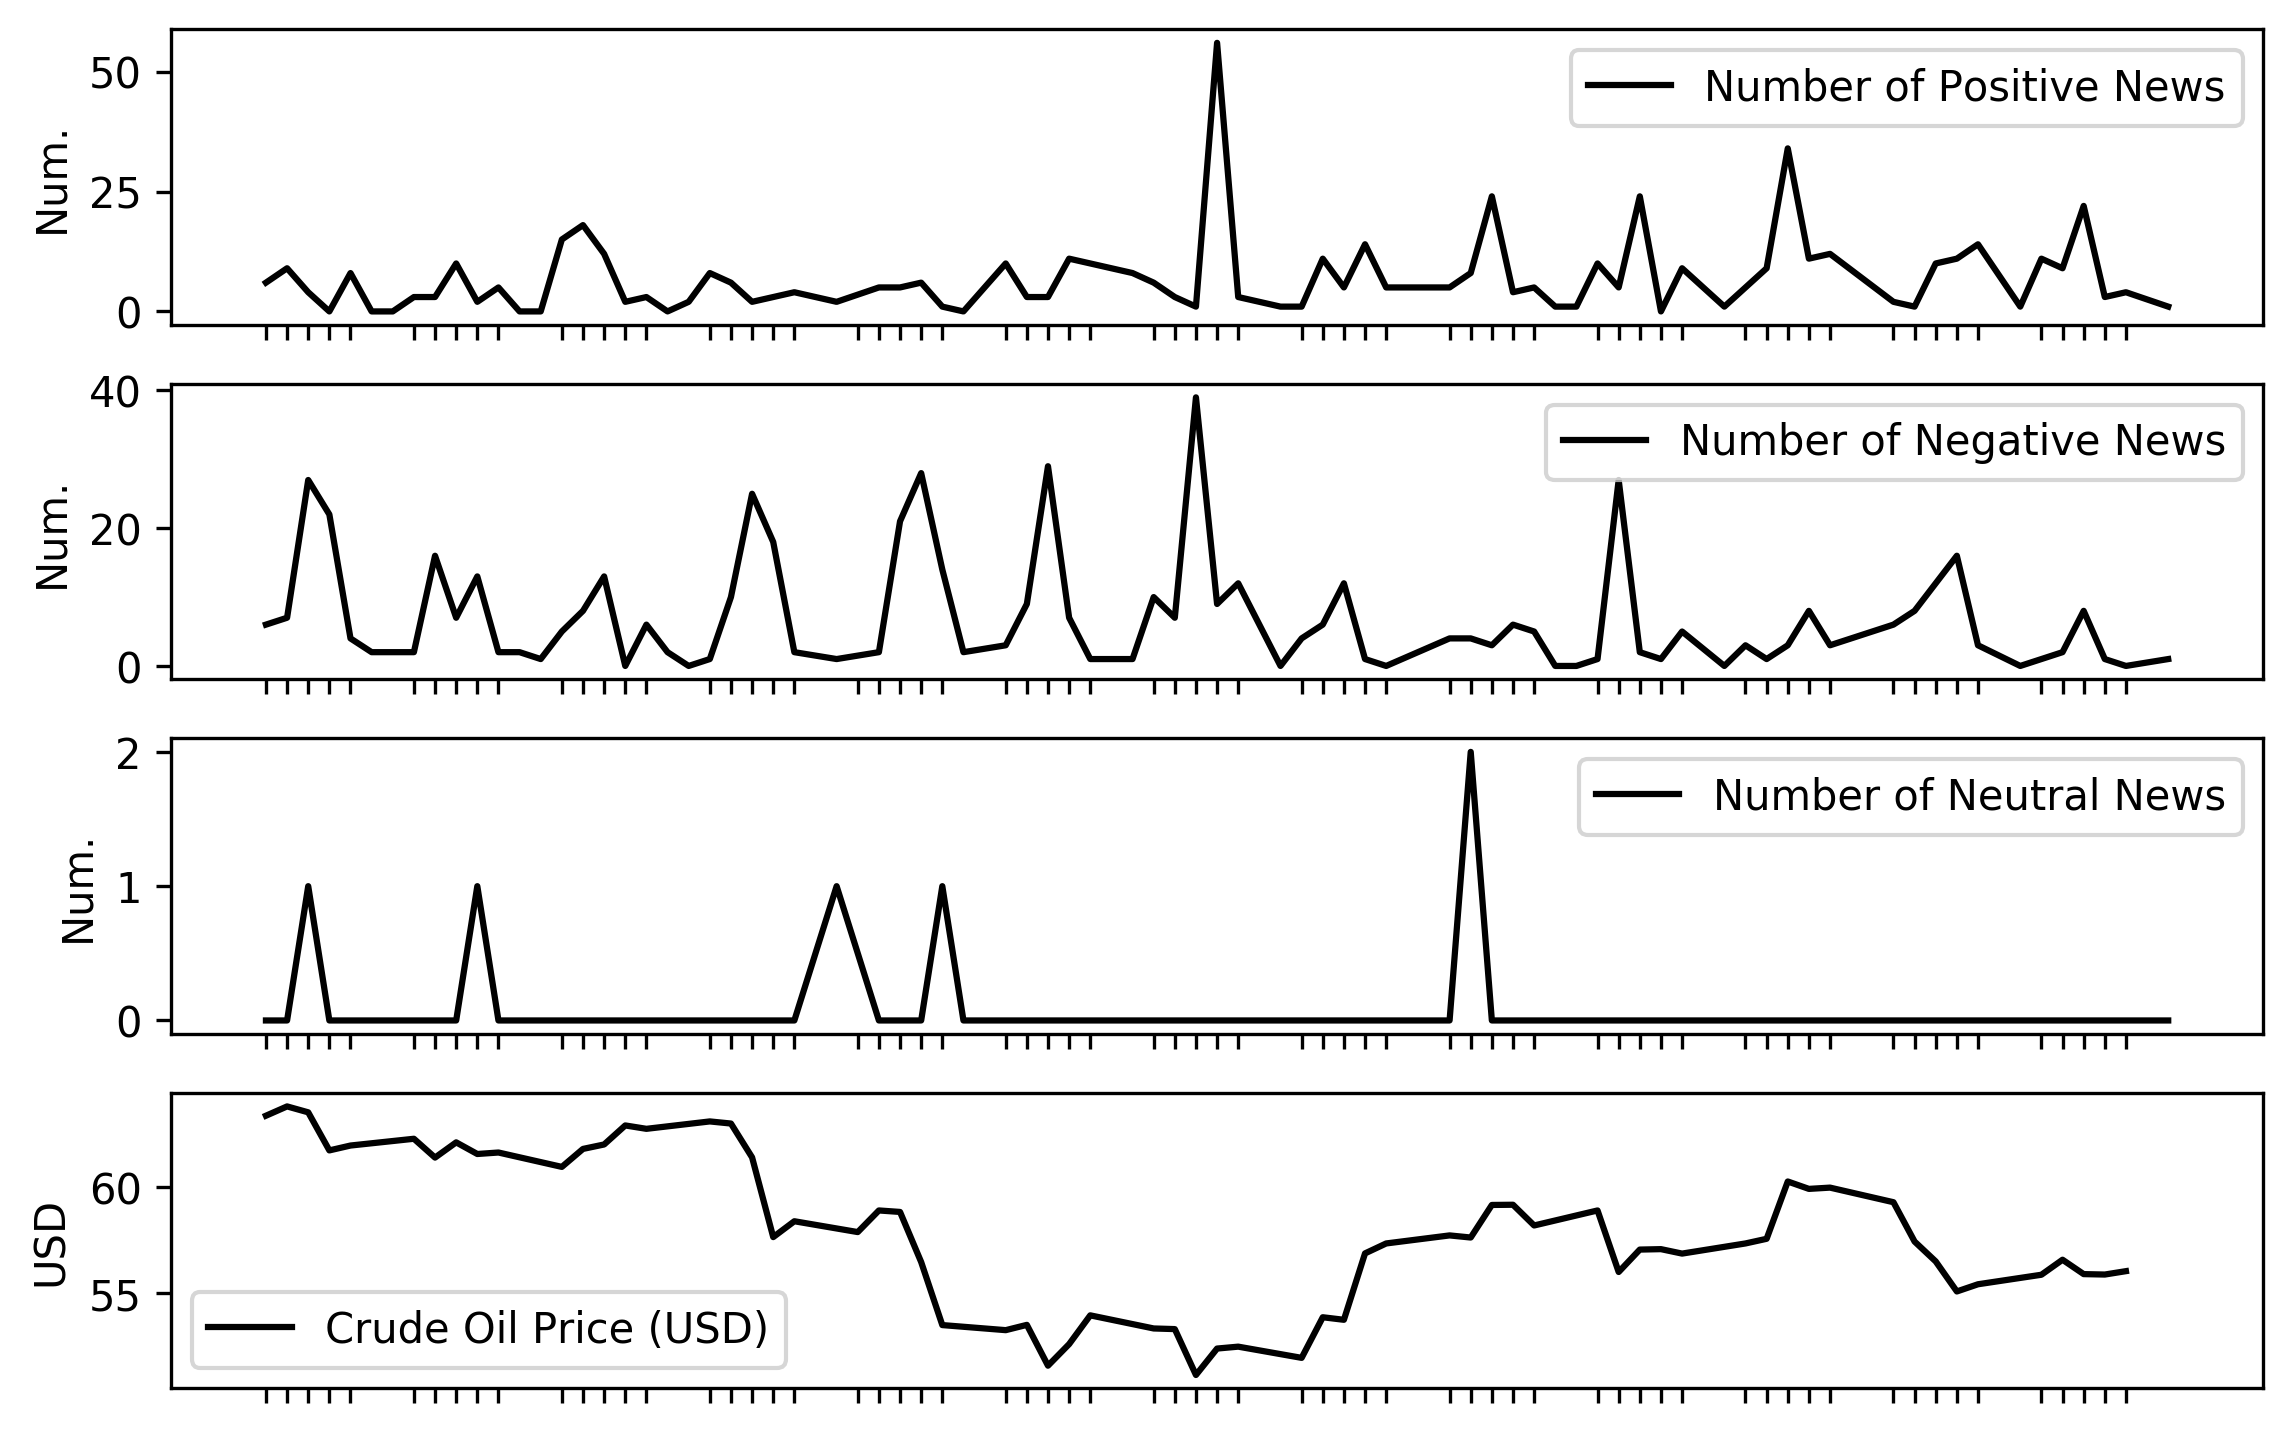
\includegraphics[width=\linewidth]{figures/case_studies/20190612_45d.png}
		\caption{}
	\end{figure}
\end{document}






















